\documentclass[aps,prx,twocolumn,superscriptaddress,nofootinbib]{revtex4-2}
\usepackage{amsmath,amssymb,bm}
\usepackage{graphicx}
\usepackage{hyperref}

% Auto-generated by build_paper_assets.py -- DO NOT EDIT BY HAND
\newcommand{\BTPlaqSimExperimentId}{\texttt{OSIRIS-BT2T-003}}
\newcommand{\BTPlaqSimExecTier}{\texttt{SIMULATED}}
\newcommand{\BTPlaqSimExactTier}{\texttt{EXACT\_STATEVECTOR}}
\newcommand{\BTPlaqProxyTier}{\texttt{PROXY}}
\newcommand{\BTPlaqSimJobId}{\texttt{null}}
\newcommand{\BTPlaqSimQpuSec}{0}
\newcommand{\BTPlaqSimSeed}{20261124}
\newcommand{\BTPlaqEncVer}{\texttt{bt2t-enc-1}}
\newcommand{\BTPlaqEncShaPrefix}{\texttt{3e3b02d13539daaf}}
\newcommand{\BTPlaqEncShaFull}{\texttt{3e3b02d13539daaf431af39056d031f777a785a556eb9da21ef4ea6097dfc4c5}}
\newcommand{\BTPlaqSimCanonicalShaPrefix}{\texttt{a913c676901a0beb}}
\newcommand{\BTPlaqSimCanonicalShaFull}{\texttt{a913c676901a0beb66743f6702424f0c1791146093946a2ba684210fbd618c0d}}
\newcommand{\BTPlaqChecksPassed}{34}
\newcommand{\BTPlaqChecksTotal}{34}
\newcommand{\BTPlaqGroupOrder}{24}
\newcommand{\BTPlaqSingleLinkQubits}{5}
\newcommand{\BTPlaqSingleLinkStates}{32}
\newcommand{\BTPlaqUnusedStates}{8}
\newcommand{\BTPlaqFourLinkGroupConfigs}{331,776}
\newcommand{\BTPlaqFourLinkGroupConfigsRaw}{331776}
\newcommand{\BTPlaqTwoLinkGroupTriples}{13,824}
\newcommand{\BTPlaqFourLinkInplaceQubits}{20}
\newcommand{\BTPlaqFourLinkInplaceStates}{1,048,576}
\newcommand{\BTPlaqFourLinkAncillaQubits}{25}
\newcommand{\BTPlaqFourLinkAncillaStates}{33,554,432}
\newcommand{\BTPlaqQubitReductionInplace}{4.0\times}
\newcommand{\BTPlaqQubitReductionAncilla}{5.0\times}
\newcommand{\BTPlaqPhysGaussSubspaceDim}{7}
\newcommand{\BTPlaqRandomGaugeConfigsChecked}{20}
\newcommand{\BTPlaqMaxGaugeDiscrepancy}{2.27 \times 10^{-15}}
\newcommand{\BTPlaqMaxGaugeDiscrepancyAscii}{2.27e-15}
\newcommand{\BTPlaqFourLinkBasisMaxErr}{2.34 \times 10^{-15}}
\newcommand{\BTPlaqTwoLinkGaugeFixedErr}{1.22 \times 10^{-15}}
\newcommand{\BTPlaqLaplacianIntertwineErr}{3.69 \times 10^{-16}}
\newcommand{\BTPlaqIsometryGramErr}{3.07 \times 10^{-12}}
\newcommand{\BTPlaqFourVertexGaussErr}{0.0}
\newcommand{\BTPlaqConjugacyClassCount}{7}
\newcommand{\BTPlaqCayleyOrder}{24}
\newcommand{\BTPlaqCayleyDiameter}{3}
\newcommand{\BTPlaqCayleyDegree}{8}
\newcommand{\BTPlaqPeterWeylCasimirDiagErr}{7.70 \times 10^{-16}}
\newcommand{\BTPlaqPeterWeylOffDiagErr}{5.94 \times 10^{-16}}
\newcommand{\BTPlaqUeQftExpmErr}{4.47 \times 10^{-16}}
\newcommand{\BTPlaqUbMatrixExpmErr}{0.0}
\newcommand{\BTPlaqUnusedCouplingNorm}{0.0}
\newcommand{\BTPlaqUnusedPropagatorErr}{0.0}
\newcommand{\BTPlaqChiClassOne}{+2.0}
\newcommand{\BTPlaqChiClassTwo}{-2.0}
\newcommand{\BTPlaqChiClassThree}{0.0}
\newcommand{\BTPlaqChiClassFour}{+1.0}
\newcommand{\BTPlaqChiClassFive}{+1.0}
\newcommand{\BTPlaqChiClassSix}{-1.0}
\newcommand{\BTPlaqChiClassSeven}{-1.0}
\newcommand{\BTPlaqVbClassOne}{0.0}
\newcommand{\BTPlaqVbClassTwo}{2.0}
\newcommand{\BTPlaqVbClassThree}{1.0}
\newcommand{\BTPlaqVbClassFour}{0.5}
\newcommand{\BTPlaqVbClassFive}{0.5}
\newcommand{\BTPlaqVbClassSix}{1.5}
\newcommand{\BTPlaqVbClassSeven}{1.5}
\newcommand{\BTPlaqHbClassOne}{-2.0}
\newcommand{\BTPlaqHbClassTwo}{+2.0}
\newcommand{\BTPlaqHbClassThree}{0.0}
\newcommand{\BTPlaqHbClassFour}{-1.0}
\newcommand{\BTPlaqHbClassFive}{-1.0}
\newcommand{\BTPlaqHbClassSix}{+1.0}
\newcommand{\BTPlaqHbClassSeven}{+1.0}
\newcommand{\BTPlaqCasimirChiZero}{0.000}
\newcommand{\BTPlaqCasimirChiOne}{2.250}
\newcommand{\BTPlaqCasimirChiTwo}{2.250}
\newcommand{\BTPlaqCasimirRhoTwoZero}{0.750}
\newcommand{\BTPlaqCasimirRhoTwoOne}{1.875}
\newcommand{\BTPlaqCasimirRhoTwoTwo}{1.875}
\newcommand{\BTPlaqCasimirRhoThree}{1.500}
\newcommand{\BTPlaqKinDimOneD}{0}
\newcommand{\BTPlaqKinDimTwoD}{2}
\newcommand{\BTPlaqKinDimThreeD}{6}
\newcommand{\BTPlaqRegimeSteps}{64}
\newcommand{\BTPlaqRegimeDt}{0.015625}
\newcommand{\BTPlaqRegimeTFinal}{1.0}
\newcommand{\BTPlaqRegimeMaxStateErr}{7.18 \times 10^{-6}}
\newcommand{\BTPlaqRegimeMaxGaussDrift}{9.06 \times 10^{-15}}
\newcommand{\BTPlaqRegimeMaxUnusedLeak}{0.0}
\newcommand{\BTPlaqWilsonWeakVacExact}{0.101207}
\newcommand{\BTPlaqWilsonWeakVacStrang}{0.101213}
\newcommand{\BTPlaqWilsonIntVacExact}{0.157329}
\newcommand{\BTPlaqWilsonIntVacStrang}{0.157331}
\newcommand{\BTPlaqWilsonStrongVacExact}{0.171556}
\newcommand{\BTPlaqWilsonStrongVacStrang}{0.171555}
\newcommand{\BTPlaqWilsonIntMagExact}{0.966455}
\newcommand{\BTPlaqWilsonIntMagStrang}{0.966454}
\newcommand{\BTPlaqLieSlopeGOne}{1.000003}
\newcommand{\BTPlaqStrangSlopeGOne}{2.000008}
\newcommand{\BTPlaqLieSlopeGHalf}{1.000011}
\newcommand{\BTPlaqStrangSlopeGHalf}{2.000033}
\newcommand{\BTPlaqLieSlopeGTwo}{1.000001}
\newcommand{\BTPlaqStrangSlopeGTwo}{2.000004}
\newcommand{\BTPlaqMaxFineStrangErr}{1.09 \times 10^{-8}}
\newcommand{\BTPlaqMaxModStrangErr}{1.11 \times 10^{-5}}
\newcommand{\BTPlaqDtStepEight}{0.125000}
\newcommand{\BTPlaqLieErrGOneStepEight}{3.35 \times 10^{-2}}
\newcommand{\BTPlaqStrangErrGOneStepEight}{5.21 \times 10^{-4}}
\newcommand{\BTPlaqDtStepSixteen}{0.062500}
\newcommand{\BTPlaqLieErrGOneStepSixteen}{1.68 \times 10^{-2}}
\newcommand{\BTPlaqStrangErrGOneStepSixteen}{1.30 \times 10^{-4}}
\newcommand{\BTPlaqDtStepThirtyTwo}{0.031250}
\newcommand{\BTPlaqLieErrGOneStepThirtyTwo}{8.38 \times 10^{-3}}
\newcommand{\BTPlaqStrangErrGOneStepThirtyTwo}{3.25 \times 10^{-5}}
\newcommand{\BTPlaqDtStepSixtyFour}{0.015625}
\newcommand{\BTPlaqLieErrGOneStepSixtyFour}{4.19 \times 10^{-3}}
\newcommand{\BTPlaqStrangErrGOneStepSixtyFour}{8.14 \times 10^{-6}}
\newcommand{\BTPlaqDtStepOneTwoEight}{0.007812}
\newcommand{\BTPlaqLieErrGOneStepOneTwoEight}{2.10 \times 10^{-3}}
\newcommand{\BTPlaqStrangErrGOneStepOneTwoEight}{2.03 \times 10^{-6}}
\newcommand{\BTPlaqDtStepTwoFiveSix}{0.003906}
\newcommand{\BTPlaqLieErrGOneStepTwoFiveSix}{1.05 \times 10^{-3}}
\newcommand{\BTPlaqStrangErrGOneStepTwoFiveSix}{5.08 \times 10^{-7}}
\newcommand{\BTPlaqDtStepFiveOneTwo}{0.001953}
\newcommand{\BTPlaqLieErrGOneStepFiveOneTwo}{5.24 \times 10^{-4}}
\newcommand{\BTPlaqStrangErrGOneStepFiveOneTwo}{1.27 \times 10^{-7}}
\newcommand{\BTPlaqDtStepOneZeroTwoFour}{0.000977}
\newcommand{\BTPlaqLieErrGOneStepOneZeroTwoFour}{2.62 \times 10^{-4}}
\newcommand{\BTPlaqStrangErrGOneStepOneZeroTwoFour}{3.18 \times 10^{-8}}
\newcommand{\BTPlaqDtStepTwoZeroFourEight}{0.000488}
\newcommand{\BTPlaqLieErrGOneStepTwoZeroFourEight}{1.31 \times 10^{-4}}
\newcommand{\BTPlaqStrangErrGOneStepTwoZeroFourEight}{7.94 \times 10^{-9}}
\newcommand{\BTPlaqCompileDt}{0.2}
\newcommand{\BTPlaqCompileGymSq}{1.0}
\newcommand{\BTPlaqUbAtaCz}{16}
\newcommand{\BTPlaqUbAtaDepth}{77}
\newcommand{\BTPlaqUbAtaSize}{79}
\newcommand{\BTPlaqUbTfCoreCz}{19}
\newcommand{\BTPlaqUbTfCoreDepth}{88}
\newcommand{\BTPlaqUbTfCoreSize}{103}
\newcommand{\BTPlaqUbTkZz}{16}
\newcommand{\BTPlaqUbTkDepth}{80}
\newcommand{\BTPlaqUbDirectErr}{1.78 \times 10^{-15}}
\newcommand{\BTPlaqUeAtaCz}{181}
\newcommand{\BTPlaqUeAtaDepth}{647}
\newcommand{\BTPlaqUeAtaSize}{893}
\newcommand{\BTPlaqUeTfCz}{312}
\newcommand{\BTPlaqUeTfDepth}{937}
\newcommand{\BTPlaqUeTfSize}{1408}
\newcommand{\BTPlaqUeDirectErr}{2.25 \times 10^{-15}}
\newcommand{\BTPlaqStrangAtaCz}{209}
\newcommand{\BTPlaqStrangAtaDepth}{790}
\newcommand{\BTPlaqStrangAtaSize}{1035}
\newcommand{\BTPlaqStrangTfCz}{350}
\newcommand{\BTPlaqStrangTfDepth}{1,080}
\newcommand{\BTPlaqStrangTfSize}{1,585}
\newcommand{\BTPlaqStrangTkZz}{208}
\newcommand{\BTPlaqStrangTkDepth}{867}
\newcommand{\BTPlaqStrangDirectErr}{2.44 \times 10^{-15}}
\newcommand{\BTPlaqDenseFiveQAtaCz}{423}
\newcommand{\BTPlaqDenseFiveQAtaDepth}{2,029}
\newcommand{\BTPlaqDenseFiveQTfCz}{613}
\newcommand{\BTPlaqDenseFiveQTfDepth}{2,543}
\newcommand{\BTPlaqDenseFiveQTkZz}{423}
\newcommand{\BTPlaqDenseFiveQTkDepth}{1,995}
\newcommand{\BTPlaqDenseVsStructAtaRatio}{2.02\times}
\newcommand{\BTPlaqDenseVsStructTfRatio}{1.75\times}
\newcommand{\BTPlaqQsdQftAtaCz}{906}
\newcommand{\BTPlaqQsdQftAtaDepth}{4,294}
\newcommand{\BTPlaqQsdQftTfCz}{1,400}
\newcommand{\BTPlaqQsdQftTfDepth}{5,473}
\newcommand{\BTPlaqFourLinkInplaceAtaCz}{21,804}
\newcommand{\BTPlaqFourLinkInplaceAtaDepth}{68,022}
\newcommand{\BTPlaqFourLinkInplaceHhCz}{47,291}
\newcommand{\BTPlaqFourLinkInplaceHhDepth}{106,526}
\newcommand{\BTPlaqFourLinkAncillaAtaCz}{28,735}
\newcommand{\BTPlaqFourLinkAncillaAtaDepth}{88,812}
\newcommand{\BTPlaqFourLinkAncillaHhCz}{62,407}
\newcommand{\BTPlaqFourLinkAncillaHhDepth}{141,698}
\newcommand{\BTPlaqCompTwentyQAtaRatio}{104.33\times}
\newcommand{\BTPlaqCompTwentyQTaOneDec}{104.3\times}
\newcommand{\BTPlaqCompTwentyQHhRatio}{135.12\times}
\newcommand{\BTPlaqCompTwentyFiveQAtaRatio}{137.49\times}
\newcommand{\BTPlaqCompTwentyFiveQHhRatio}{178.31\times}
\newcommand{\BTPlaqCompTwentyFiveQHhOneDec}{178.3\times}
\newcommand{\BTPlaqFezProtocolId}{\texttt{OSIRIS-BT2T-003-FEZ}}
\newcommand{\BTPlaqFezExecTier}{\texttt{HARDWARE_ATTESTED}}
\newcommand{\BTPlaqFezBackend}{\texttt{ibm\_fez}}
\newcommand{\BTPlaqFezJobId}{\texttt{dc38nreq4uuc73a6g0k0}}
\newcommand{\BTPlaqFezWindowOneJobId}{\texttt{dc35e35s2omc738cvcug}}
\newcommand{\BTPlaqFezQpuSec}{19}
\newcommand{\BTPlaqFezTotalPubs}{240}
\newcommand{\BTPlaqFezShotsPerPub}{256}
\newcommand{\BTPlaqFezTotalShots}{61,440}
\newcommand{\BTPlaqFezTotalShotsRaw}{61440}
\newcommand{\BTPlaqFezBlocks}{3}
\newcommand{\BTPlaqFezPubsPerBlock}{80}
\newcommand{\BTPlaqFezNumPlacements}{10}
\newcommand{\BTPlaqFezTotalTransmons}{50}
\newcommand{\BTPlaqFezWriteAheadCommit}{\texttt{82cfd46a}}
\newcommand{\BTPlaqFezWriteAheadCommitFull}{\texttt{82cfd46a8ef091fbb6919f5112578d8e657eef7a}}
\newcommand{\BTPlaqFezQpyShaPrefix}{\texttt{349a7ab40a1a55db}}
\newcommand{\BTPlaqFezQpyShaFull}{\texttt{349a7ab40a1a55db6ca85dbfd27c24f75aa3e4c67c20accad82a7a41b2c87b9a}}
\newcommand{\BTPlaqFezRawCountsShaPrefix}{\texttt{4667adc71b3af9b7}}
\newcommand{\BTPlaqFezRawCountsShaFull}{\texttt{4667adc71b3af9b7dd3c9dff1fde9d4d6acaf768597992bfbc39bbde2c0abeb3}}
\newcommand{\BTPlaqFezPreregShaPrefix}{\texttt{da07a4f45ff99442}}
\newcommand{\BTPlaqFezCzIdentity}{0}
\newcommand{\BTPlaqFezCzEchoProbe}{16}
\newcommand{\BTPlaqFezCzCenterStruct}{40}
\newcommand{\BTPlaqFezCzCenterGeneric}{2,727}
\newcommand{\BTPlaqFezCzCenterGenericRaw}{2727}
\newcommand{\BTPlaqFezCzHurwitzStruct}{48}
\newcommand{\BTPlaqFezCzImagNull}{40}
\newcommand{\BTPlaqFezCzUnusedNull}{40}
\newcommand{\BTPlaqFezCzClifford}{30}
\newcommand{\BTPlaqFezCzMirror}{24}
\newcommand{\BTPlaqFezCzReductionRatio}{68.18\times}
\newcommand{\BTPlaqFezCoreCzReductionRatio}{143.53\times}
\newcommand{\BTPlaqRoutedYCenterInv}{2}
\newcommand{\BTPlaqRoutedBitsCenterInv}{\texttt{00010}}
\newcommand{\BTPlaqRoutedYHurwitzInv}{4}
\newcommand{\BTPlaqRoutedBitsHurwitzInv}{\texttt{00100}}
\newcommand{\BTPlaqRoutedYImagNull}{1}
\newcommand{\BTPlaqRoutedBitsImagNull}{\texttt{00001}}
\newcommand{\BTPlaqRoutedYUnusedNull}{12}
\newcommand{\BTPlaqRoutedBitsUnusedNull}{\texttt{01100}}
\newcommand{\BTPlaqRoutedYClifford}{21}
\newcommand{\BTPlaqRoutedYMirror}{25}
\newcommand{\BTPlaqIdealOne}{1.000000}
\newcommand{\BTPlaqIdealHalf}{0.500000}
\newcommand{\BTPlaqIdealZero}{0.000000}
\newcommand{\BTPlaqIdealCosSqPiEight}{0.853553}
\newcommand{\BTPlaqIdealCosSqThreePiEight}{0.146447}
\newcommand{\BTPlaqPidZeroCenterTZero}{0.876302}
\newcommand{\BTPlaqPidZeroCenterPiEight}{0.411458}
\newcommand{\BTPlaqPidZeroCenterPiFourPlus}{0.057292}
\newcommand{\BTPlaqPidZeroCenterPiFourMinus}{0.850260}
\newcommand{\BTPlaqPidZeroCenterPiFourMinusPct}{85.03\%}
\newcommand{\BTPlaqPidZeroCenterPiTwo}{0.841146}
\newcommand{\BTPlaqPidZeroPearsonCenter}{0.997576}
\newcommand{\BTPlaqPidZeroCenterGenericMinus}{0.041667}
\newcommand{\BTPlaqPidZeroCenterStructAdv}{0.808594}
\newcommand{\BTPlaqPidZeroCenterStructAdvPp}{80.86}
\newcommand{\BTPlaqPidZeroCenterStructFidelityRatio}{20.41\times}
\newcommand{\BTPlaqPidZeroHurwitzTZero}{0.829427}
\newcommand{\BTPlaqPidZeroHurwitzPiEight}{0.669271}
\newcommand{\BTPlaqPidZeroHurwitzPiFour}{0.404948}
\newcommand{\BTPlaqPidZeroHurwitzThreePiEight}{0.130208}
\newcommand{\BTPlaqPidZeroHurwitzPiTwoPlus}{0.050781}
\newcommand{\BTPlaqPidZeroHurwitzPiTwoMinus}{0.796875}
\newcommand{\BTPlaqPidZeroHurwitzPiTwoMinusPct}{79.69\%}
\newcommand{\BTPlaqPidZeroPearsonHurwitz}{0.997940}
\newcommand{\BTPlaqPidZeroImagNullSurv}{0.861979}
\newcommand{\BTPlaqPidZeroUnusedNullSurv}{0.785156}
\newcommand{\BTPlaqPidOneCenterTZero}{0.548177}
\newcommand{\BTPlaqPidOneCenterPiEight}{0.279948}
\newcommand{\BTPlaqPidOneCenterPiFourPlus}{0.045573}
\newcommand{\BTPlaqPidOneCenterPiFourMinus}{0.539062}
\newcommand{\BTPlaqPidOneCenterPiTwo}{0.553385}
\newcommand{\BTPlaqPidOnePearsonCenter}{0.999283}
\newcommand{\BTPlaqPidOneCenterGenericMinus}{0.046875}
\newcommand{\BTPlaqPidOneCenterStructAdv}{0.492188}
\newcommand{\BTPlaqPidOneCenterStructFidelityRatio}{11.50\times}
\newcommand{\BTPlaqPidOneHurwitzTZero}{0.460938}
\newcommand{\BTPlaqPidOneHurwitzPiEight}{0.393229}
\newcommand{\BTPlaqPidOneHurwitzPiFour}{0.290365}
\newcommand{\BTPlaqPidOneHurwitzThreePiEight}{0.239583}
\newcommand{\BTPlaqPidOneHurwitzPiTwoPlus}{0.221354}
\newcommand{\BTPlaqPidOneHurwitzPiTwoMinus}{0.361979}
\newcommand{\BTPlaqPidOnePearsonHurwitz}{0.977581}
\newcommand{\BTPlaqPidOneImagNullSurv}{0.524740}
\newcommand{\BTPlaqPidOneUnusedNullSurv}{0.380208}
\newcommand{\BTPlaqEchoNumWindows}{2}
\newcommand{\BTPlaqEchoElapsedHours}{3.763}
\newcommand{\BTPlaqDriftedHubQubit}{7}
\newcommand{\BTPlaqWOnePidOneIdFid}{0.962240}
\newcommand{\BTPlaqWTwoPidOneIdFid}{0.677083}
\newcommand{\BTPlaqWOnePidOneEcho}{0.815104}
\newcommand{\BTPlaqWTwoPidOneEcho}{0.562500}
\newcommand{\BTPlaqQSevenExcitation}{0.311198}
\newcommand{\BTPlaqQSevenExcitationPct}{31.12\%}
\newcommand{\BTPlaqWOneSpearmanCal}{0.781818}
\newcommand{\BTPlaqWOneSpearmanEcho}{0.721212}
\newcommand{\BTPlaqWOneSpearmanNormEcho}{0.903030}
\newcommand{\BTPlaqWOneRegretCal}{0.000000}
\newcommand{\BTPlaqWOneRegretEcho}{0.000000}
\newcommand{\BTPlaqWTwoSpearmanCal}{0.454545}
\newcommand{\BTPlaqWTwoSpearmanEcho}{0.948333}
\newcommand{\BTPlaqWTwoSpearmanNormEcho}{0.745455}
\newcommand{\BTPlaqWTwoDeltaSpearman}{0.493787}
\newcommand{\BTPlaqWTwoRegretCal}{0.361002}
\newcommand{\BTPlaqWTwoRegretCalPp}{36.10}
\newcommand{\BTPlaqWTwoRegretEcho}{0.000000}
\newcommand{\BTPlaqWTwoRegretNormEcho}{0.158854}
\newcommand{\BTPlaqTwoWinMeanSpearmanCal}{0.618182}
\newcommand{\BTPlaqTwoWinMeanSpearmanEcho}{0.834772}
\newcommand{\BTPlaqTwoWinMeanSpearmanNormEcho}{0.824242}
\newcommand{\BTPlaqTwoWinMeanDeltaSpearman}{0.216591}
\newcommand{\BTPlaqPooledSpearmanCalAll}{0.537362}
\newcommand{\BTPlaqPooledSpearmanEchoAll}{0.767206}
\newcommand{\BTPlaqPooledSpearmanCalClfMir}{0.670193}
\newcommand{\BTPlaqPooledSpearmanEchoClfMir}{0.889808}
\newcommand{\BTPlaqRhoCalClifford}{0.539}
\newcommand{\BTPlaqRhoEchoClifford}{0.979}
\newcommand{\BTPlaqDeltaRhoClifford}{0.439}
\newcommand{\BTPlaqRhoCalMirror}{0.565352}
\newcommand{\BTPlaqRhoEchoMirror}{0.929878}
\newcommand{\BTPlaqDeltaRhoMirror}{0.364526}
\newcommand{\BTPlaqRhoCalClfMir}{0.575758}
\newcommand{\BTPlaqRhoEchoClfMir}{0.930095}
\newcommand{\BTPlaqDeltaRhoClfMir}{0.354338}
\newcommand{\BTPlaqRhoCalCenter}{0.503030}
\newcommand{\BTPlaqRhoEchoCenter}{0.826752}
\newcommand{\BTPlaqDeltaRhoCenter}{0.323721}
\newcommand{\BTPlaqRhoCalHurwitz}{0.455929}
\newcommand{\BTPlaqRhoEchoHurwitz}{0.890244}
\newcommand{\BTPlaqDeltaRhoHurwitz}{0.434315}
\newcommand{\BTPlaqRhoCalPlaqTwoW}{0.527273}
\newcommand{\BTPlaqRhoEchoPlaqTwoW}{0.844989}
\newcommand{\BTPlaqDeltaRhoPlaqTwoW}{0.317716}
\newcommand{\BTPlaqPidZeroQubits}{\texttt{[21, 22, 23, 16, 24]}}
\newcommand{\BTPlaqPidZeroCalScore}{-0.139835}
\newcommand{\BTPlaqPidZeroCalRank}{2}
\newcommand{\BTPlaqPidZeroIdZeroCz}{0.976562}
\newcommand{\BTPlaqPidZeroEchoSixteenCz}{0.858073}
\newcommand{\BTPlaqPidZeroEchoRank}{1}
\newcommand{\BTPlaqPidZeroNormEcho}{0.878667}
\newcommand{\BTPlaqPidZeroUbCenter}{0.850260}
\newcommand{\BTPlaqPidZeroUbHurwitz}{0.796875}
\newcommand{\BTPlaqPidZeroPlaqComp}{0.823568}
\newcommand{\BTPlaqPidZeroClifford}{0.761719}
\newcommand{\BTPlaqPidZeroMirror}{0.837240}
\newcommand{\BTPlaqPidZeroClfMirComp}{0.799479}
\newcommand{\BTPlaqPidZeroHeldoutComp}{0.811523}
\newcommand{\BTPlaqPidOneQubits}{\texttt{[5, 6, 7, 8, 17]}}
\newcommand{\BTPlaqPidOneCalScore}{-0.103649}
\newcommand{\BTPlaqPidOneCalRank}{1}
\newcommand{\BTPlaqPidOneIdZeroCz}{0.677083}
\newcommand{\BTPlaqPidOneEchoSixteenCz}{0.562500}
\newcommand{\BTPlaqPidOneEchoRank}{8}
\newcommand{\BTPlaqPidOneNormEcho}{0.830769}
\newcommand{\BTPlaqPidOneUbCenter}{0.539062}
\newcommand{\BTPlaqPidOneUbHurwitz}{0.361979}
\newcommand{\BTPlaqPidOnePlaqComp}{0.450521}
\newcommand{\BTPlaqPidOneClifford}{0.380208}
\newcommand{\BTPlaqPidOneMirror}{0.520833}
\newcommand{\BTPlaqPidOneClfMirComp}{0.450521}
\newcommand{\BTPlaqPidOneHeldoutComp}{0.450521}
\newcommand{\BTPlaqPidTwoQubits}{\texttt{[9, 10, 11, 12, 18]}}
\newcommand{\BTPlaqPidTwoCalScore}{-0.393731}
\newcommand{\BTPlaqPidTwoCalRank}{8}
\newcommand{\BTPlaqPidTwoIdZeroCz}{0.950521}
\newcommand{\BTPlaqPidTwoEchoSixteenCz}{0.697917}
\newcommand{\BTPlaqPidTwoEchoRank}{5}
\newcommand{\BTPlaqPidTwoNormEcho}{0.734247}
\newcommand{\BTPlaqPidTwoUbCenter}{0.710938}
\newcommand{\BTPlaqPidTwoUbHurwitz}{0.503906}
\newcommand{\BTPlaqPidTwoPlaqComp}{0.607422}
\newcommand{\BTPlaqPidTwoClifford}{0.500000}
\newcommand{\BTPlaqPidTwoMirror}{0.630208}
\newcommand{\BTPlaqPidTwoClfMirComp}{0.565104}
\newcommand{\BTPlaqPidTwoHeldoutComp}{0.586263}
\newcommand{\BTPlaqPidThreeQubits}{\texttt{[27, 28, 29, 30, 38]}}
\newcommand{\BTPlaqPidThreeCalScore}{-0.430006}
\newcommand{\BTPlaqPidThreeCalRank}{9}
\newcommand{\BTPlaqPidThreeIdZeroCz}{0.976562}
\newcommand{\BTPlaqPidThreeEchoSixteenCz}{0.411458}
\newcommand{\BTPlaqPidThreeEchoRank}{9}
\newcommand{\BTPlaqPidThreeNormEcho}{0.421333}
\newcommand{\BTPlaqPidThreeUbCenter}{0.630208}
\newcommand{\BTPlaqPidThreeUbHurwitz}{0.563802}
\newcommand{\BTPlaqPidThreePlaqComp}{0.597005}
\newcommand{\BTPlaqPidThreeClifford}{0.294271}
\newcommand{\BTPlaqPidThreeMirror}{0.375000}
\newcommand{\BTPlaqPidThreeClfMirComp}{0.334635}
\newcommand{\BTPlaqPidThreeHeldoutComp}{0.465820}
\newcommand{\BTPlaqPidFourQubits}{\texttt{[31, 32, 33, 34, 39]}}
\newcommand{\BTPlaqPidFourCalScore}{-4.147669}
\newcommand{\BTPlaqPidFourCalRank}{10}
\newcommand{\BTPlaqPidFourIdZeroCz}{0.679688}
\newcommand{\BTPlaqPidFourEchoSixteenCz}{0.209635}
\newcommand{\BTPlaqPidFourEchoRank}{10}
\newcommand{\BTPlaqPidFourNormEcho}{0.308429}
\newcommand{\BTPlaqPidFourUbCenter}{0.031250}
\newcommand{\BTPlaqPidFourUbHurwitz}{0.035156}
\newcommand{\BTPlaqPidFourPlaqComp}{0.033203}
\newcommand{\BTPlaqPidFourClifford}{0.031250}
\newcommand{\BTPlaqPidFourMirror}{0.126302}
\newcommand{\BTPlaqPidFourClfMirComp}{0.078776}
\newcommand{\BTPlaqPidFourHeldoutComp}{0.055990}
\newcommand{\BTPlaqPidFiveQubits}{\texttt{[43, 42, 41, 36, 40]}}
\newcommand{\BTPlaqPidFiveCalScore}{-0.345024}
\newcommand{\BTPlaqPidFiveCalRank}{7}
\newcommand{\BTPlaqPidFiveIdZeroCz}{0.855469}
\newcommand{\BTPlaqPidFiveEchoSixteenCz}{0.733073}
\newcommand{\BTPlaqPidFiveEchoRank}{3}
\newcommand{\BTPlaqPidFiveNormEcho}{0.856925}
\newcommand{\BTPlaqPidFiveUbCenter}{0.751302}
\newcommand{\BTPlaqPidFiveUbHurwitz}{0.640625}
\newcommand{\BTPlaqPidFivePlaqComp}{0.695964}
\newcommand{\BTPlaqPidFiveClifford}{0.631510}
\newcommand{\BTPlaqPidFiveMirror}{0.647135}
\newcommand{\BTPlaqPidFiveClfMirComp}{0.639323}
\newcommand{\BTPlaqPidFiveHeldoutComp}{0.667643}
\newcommand{\BTPlaqPidSixQubits}{\texttt{[25, 37, 45, 44, 46]}}
\newcommand{\BTPlaqPidSixCalScore}{-0.156496}
\newcommand{\BTPlaqPidSixCalRank}{3}
\newcommand{\BTPlaqPidSixIdZeroCz}{0.949219}
\newcommand{\BTPlaqPidSixEchoSixteenCz}{0.832031}
\newcommand{\BTPlaqPidSixEchoRank}{2}
\newcommand{\BTPlaqPidSixNormEcho}{0.876543}
\newcommand{\BTPlaqPidSixUbCenter}{0.846354}
\newcommand{\BTPlaqPidSixUbHurwitz}{0.720052}
\newcommand{\BTPlaqPidSixPlaqComp}{0.783203}
\newcommand{\BTPlaqPidSixClifford}{0.701823}
\newcommand{\BTPlaqPidSixMirror}{0.723958}
\newcommand{\BTPlaqPidSixClfMirComp}{0.712891}
\newcommand{\BTPlaqPidSixHeldoutComp}{0.748047}
\newcommand{\BTPlaqPidSevenQubits}{\texttt{[49, 50, 51, 52, 58]}}
\newcommand{\BTPlaqPidSevenCalScore}{-0.163459}
\newcommand{\BTPlaqPidSevenCalRank}{4}
\newcommand{\BTPlaqPidSevenIdZeroCz}{0.927083}
\newcommand{\BTPlaqPidSevenEchoSixteenCz}{0.686198}
\newcommand{\BTPlaqPidSevenEchoRank}{7}
\newcommand{\BTPlaqPidSevenNormEcho}{0.740169}
\newcommand{\BTPlaqPidSevenUbCenter}{0.755208}
\newcommand{\BTPlaqPidSevenUbHurwitz}{0.638021}
\newcommand{\BTPlaqPidSevenPlaqComp}{0.696615}
\newcommand{\BTPlaqPidSevenClifford}{0.572917}
\newcommand{\BTPlaqPidSevenMirror}{0.630208}
\newcommand{\BTPlaqPidSevenClfMirComp}{0.601562}
\newcommand{\BTPlaqPidSevenHeldoutComp}{0.649089}
\newcommand{\BTPlaqPidEightQubits}{\texttt{[63, 62, 61, 60, 76]}}
\newcommand{\BTPlaqPidEightCalScore}{-0.231744}
\newcommand{\BTPlaqPidEightCalRank}{5}
\newcommand{\BTPlaqPidEightIdZeroCz}{0.880208}
\newcommand{\BTPlaqPidEightEchoSixteenCz}{0.697917}
\newcommand{\BTPlaqPidEightEchoRank}{6}
\newcommand{\BTPlaqPidEightNormEcho}{0.792899}
\newcommand{\BTPlaqPidEightUbCenter}{0.714844}
\newcommand{\BTPlaqPidEightUbHurwitz}{0.639323}
\newcommand{\BTPlaqPidEightPlaqComp}{0.677083}
\newcommand{\BTPlaqPidEightClifford}{0.609375}
\newcommand{\BTPlaqPidEightMirror}{0.692708}
\newcommand{\BTPlaqPidEightClfMirComp}{0.651042}
\newcommand{\BTPlaqPidEightHeldoutComp}{0.664062}
\newcommand{\BTPlaqPidNineQubits}{\texttt{[67, 66, 65, 64, 77]}}
\newcommand{\BTPlaqPidNineCalScore}{-0.251468}
\newcommand{\BTPlaqPidNineCalRank}{6}
\newcommand{\BTPlaqPidNineIdZeroCz}{0.807292}
\newcommand{\BTPlaqPidNineEchoSixteenCz}{0.714844}
\newcommand{\BTPlaqPidNineEchoRank}{4}
\newcommand{\BTPlaqPidNineNormEcho}{0.885484}
\newcommand{\BTPlaqPidNineUbCenter}{0.697917}
\newcommand{\BTPlaqPidNineUbHurwitz}{0.638021}
\newcommand{\BTPlaqPidNinePlaqComp}{0.667969}
\newcommand{\BTPlaqPidNineClifford}{0.611979}
\newcommand{\BTPlaqPidNineMirror}{0.662760}
\newcommand{\BTPlaqPidNineClfMirComp}{0.637370}
\newcommand{\BTPlaqPidNineHeldoutComp}{0.652669}


\begin{document}

\title{Maximal-Tree Gauge-Fixed Binary Tetrahedral ($2T \subset SU(2)$) Kogut--Susskind Plaquette Dynamics, \BTPlaqFezCzReductionRatio\ Walsh--Hadamard Magnetic Gate Compression, and Live Two-Window \texttt{OSIRIS-ECHO} Intra-Calibration Drift Catch Across \BTPlaqFezTotalTransmons\ Transmons on \BTPlaqFezBackend}

\author{Devin Phillip Davis}
\affiliation{Agile Defense Systems LLC, Lexington, Kentucky, USA}
\date{November 25, 2026}

\begin{abstract}
Digital quantum simulation of $(2+1)$-dimensional non-abelian $SU(2)$ Kogut--Susskind lattice Yang--Mills theory over the binary tetrahedral gauge group $2T \cong SL(2,\mathbb{F}_3)$ of order $|2T| = \BTPlaqGroupOrder$ faces prohibitive register and entangling-gate scaling when unfixed four-link single-plaquette Hilbert spaces ($|2T|^4 = 24^4 = \BTPlaqFourLinkGroupConfigs$ group configurations embedded in $\BTPlaqFourLinkInplaceQubits$ qubits of dimension $32^4 = \BTPlaqFourLinkInplaceStates$, or $\BTPlaqFourLinkAncillaQubits$ qubits of dimension $32^5 = \BTPlaqFourLinkAncillaStates$ with a five-qubit holonomy workspace register) are evolved directly. Under frozen five-qubit Hurwitz quaternion encoding \BTPlaqEncVer\ (SHA-256 prefix \BTPlaqEncShaPrefix), we present a dual-manifest investigation joining exhaustive offline algebraic and Trotter--Suzuki verification (\BTPlaqSimExperimentId; execution tier \BTPlaqSimExecTier\ / \BTPlaqSimExactTier, $\BTPlaqChecksPassed/\BTPlaqChecksTotal$ checks, \texttt{provider\_job\_id:} \BTPlaqSimJobId, \BTPlaqSimQpuSec\,s QPU) with write-ahead hardware execution across $\BTPlaqFezTotalTransmons$ physical transmons on the $156$-qubit IBM Heron~r2 processor \BTPlaqFezBackend\ (\BTPlaqFezProtocolId; execution tier \BTPlaqFezExecTier, \texttt{provider\_job\_id:} \BTPlaqFezJobId, $\BTPlaqFezTotalPubs$ PUBs $\times \BTPlaqFezShotsPerPub = \BTPlaqFezTotalShots$ shots across $K = \BTPlaqFezNumPlacements$ disjoint \texttt{T5} heavy-hex subgraphs, write-ahead staged at commit \BTPlaqFezWriteAheadCommit, QPY SHA-256 prefix \BTPlaqFezQpyShaPrefix, raw-counts SHA-256 prefix \BTPlaqFezRawCountsShaPrefix). First, maximal-tree gauge fixing collapses the four-link Kogut--Susskind plaquette space from $\BTPlaqFourLinkGroupConfigs$ configurations to $\BTPlaqGroupOrder$ physical holonomy states on $\BTPlaqSingleLinkQubits$ qubits ($\BTPlaqSingleLinkStates$-dimensional register with $\BTPlaqGroupOrder$ active states, $\BTPlaqUnusedStates$ decoupled unused codewords, and a $\BTPlaqPhysGaussSubspaceDim$-dimensional conjugation-invariant physical Gauss-law subspace), matching unfixed four-link evolution across $\BTPlaqRandomGaugeConfigsChecked$ random gauge configurations to $\BTPlaqMaxGaugeDiscrepancy$. The exact magnetic plaquette potential $V_B(U) = \tfrac{1}{2}(2 - \operatorname{Re}\chi_{2D}(U)) \in \{0, \tfrac{1}{2}, 1, \tfrac{3}{2}, 2\}$ across the $\BTPlaqConjugacyClassCount$ conjugacy classes $C_1,\dots,C_7$ compiles via a five-qubit diagonal Walsh--Hadamard Gray-code phase circuit to $\BTPlaqUbAtaCz$ \texttt{CZ} gates (all-to-all) or $\BTPlaqUbTfCoreCz$ core \texttt{CZ} gates on heavy-hex \texttt{T5} ($\BTPlaqFezCzCenterStruct$ total \texttt{CZ} including state preparation and measurement versus $\BTPlaqFezCzCenterGeneric$ \texttt{CZ} for generic dense $32\times 32$ QFT-conjugated \texttt{UnitaryGate} synthesis: a \BTPlaqFezCzReductionRatio\ native \texttt{CZ} reduction on \BTPlaqFezBackend). Combined with the non-abelian electric kinetic operator $T_E = \sum_\rho d_\rho(d_\rho - 1)\Pi_\rho$ ($\BTPlaqKinDimOneD$ on $3\times 1\mathrm{D}$ $A_3$, $\BTPlaqKinDimTwoD$ on $3\times 2\mathrm{D}$ $E_{1,2,3}$, $\BTPlaqKinDimThreeD$ on $1\times 3\mathrm{D}$ $T$) and continuum-calibrated $SU(2)$ Casimir spectrum $c_2(\rho) \in \{0, \tfrac{3}{4}, \tfrac{3}{2}, \tfrac{15}{8}, \tfrac{9}{4}\}$ diagonal in the $32\times 32$ Peter--Weyl basis $\widetilde{F}_{2T}$, second-order Strang splitting $S_2(\Delta t) = U_B(\Delta t/2)\widetilde{F}_{2T}^\dagger D_E(\Delta t)\widetilde{F}_{2T} U_B(\Delta t/2)$ compiles to $\BTPlaqStrangAtaCz$ \texttt{CZ} (all-to-all) and $\BTPlaqStrangTfCz$ \texttt{CZ} (heavy-hex \texttt{T5})---\BTPlaqCompTwentyQAtaRatio\ to \BTPlaqCompTwentyFiveQHhRatio\ fewer \texttt{CZ} gates than unfixed $\BTPlaqFourLinkInplaceQubits$Q/$\BTPlaqFourLinkAncillaQubits$Q four-link Trotterization ($\BTPlaqFourLinkInplaceAtaCz$ to $\BTPlaqFourLinkAncillaHhCz$ \texttt{CZ})---with empirical log-log Strang convergence slope $\BTPlaqStrangSlopeGOne$. Second, on Echo-selected top-1 placement \texttt{pid=0} (\BTPlaqPidZeroQubits) on \BTPlaqFezBackend, the $\BTPlaqUbTfCoreCz$-\texttt{CZ} core magnetic propagator resolves both non-abelian character frequencies: in the Center sector ($\Delta\chi_{2D} = 4$, theoretical $P_{|+\rangle}(\tau) = \cos^2(2\tau)$), measured survival tracks $[\BTPlaqPidZeroCenterTZero, \BTPlaqPidZeroCenterPiEight, \BTPlaqPidZeroCenterPiFourPlus, \BTPlaqPidZeroCenterPiTwo]$ (Pearson $r = \BTPlaqPidZeroPearsonCenter$) with $P_{|-\rangle}(\pi/4) = \BTPlaqPidZeroCenterPiFourMinus$ (\BTPlaqPidZeroCenterPiFourMinusPct\ inversion into routed \BTPlaqRoutedBitsCenterInv) versus $\BTPlaqPidZeroCenterGenericMinus$ for the $\BTPlaqFezCzCenterGeneric$-\texttt{CZ} generic dense comparator ($+\BTPlaqPidZeroCenterStructAdv = \BTPlaqPidZeroCenterStructAdvPp$ percentage-point / \BTPlaqPidZeroCenterStructFidelityRatio\ structured compiler fidelity advantage); in the Hurwitz half-frequency sector ($\Delta\chi_{2D} = 2$, theoretical $P_{\Phi^+}(\tau) = \cos^2\tau$), measured survival tracks $[\BTPlaqPidZeroHurwitzTZero, \BTPlaqPidZeroHurwitzPiEight, \BTPlaqPidZeroHurwitzPiFour, \BTPlaqPidZeroHurwitzThreePiEight, \BTPlaqPidZeroHurwitzPiTwoPlus]$ (Pearson $r = \BTPlaqPidZeroPearsonHurwitz$) with $P_{\Phi^-}(\pi/2) = \BTPlaqPidZeroHurwitzPiTwoMinus$ (\BTPlaqPidZeroHurwitzPiTwoMinusPct\ inversion into routed \BTPlaqRoutedBitsHurwitzInv); and zero-differential-character null controls ($\Delta\chi_{2D} = 0$ at $\tau = \pi/4$) preserve $\BTPlaqPidZeroImagNullSurv$ on imaginary-$Q_8$ $|\mathbf{i}\rangle$ (\BTPlaqRoutedBitsImagNull) and $\BTPlaqPidZeroUnusedNullSurv$ on unused-$8$ $|y=24\rangle$ (\BTPlaqRoutedBitsUnusedNull). Third, across a live two-window ($N_{\mathrm{windows}} = \BTPlaqEchoNumWindows$, $+\BTPlaqEchoElapsedHours$\,h) placement campaign spanning Window~1 (job \BTPlaqFezWindowOneJobId) and Window~2 (job \BTPlaqFezJobId), hub transmon Q\BTPlaqDriftedHubQubit\ of \texttt{pid=1} (\BTPlaqPidOneQubits) suffered an unflagged $+\BTPlaqQSevenExcitationPct$ $|0\rangle\to|1\rangle$ SPAM/readout drift excursion (\texttt{IDENTITY\_CTRL\_0CZ} dropping $\BTPlaqWOnePidOneIdFid \to \BTPlaqWTwoPidOneIdFid$, \texttt{ECHO\_PROBE\_16CZ} dropping $\BTPlaqWOnePidOneEcho \to \BTPlaqWTwoPidOneEcho$). Published calibration remained frozen at the stale Window~1 ranking (\texttt{pid=1} at \#1), collapsing in Window~2 to Spearman $\rho_{\mathrm{cal}} = +\BTPlaqWTwoSpearmanCal$ with $\BTPlaqWTwoRegretCal$ top-1 selection regret, whereas live \texttt{ECHO\_PROBE\_16CZ} detected the \texttt{pid=1} collapse in real time, switched \#1 selection to \texttt{pid=0}, and achieved $\rho_{\mathrm{echo}} = +\BTPlaqWTwoSpearmanEcho$ ($\Delta\rho = +\BTPlaqWTwoDeltaSpearman$ over calibration) with $\BTPlaqWTwoRegretEcho$ top-1 selection regret across both windows (two-window mean $\bar{\rho}_{\mathrm{echo}} = +\BTPlaqTwoWinMeanSpearmanEcho$ versus $\bar{\rho}_{\mathrm{cal}} = +\BTPlaqTwoWinMeanSpearmanCal$, $\Delta\bar{\rho} = +\BTPlaqTwoWinMeanDeltaSpearman$).
\end{abstract}

\maketitle

\section{Introduction and Provenance Architecture}

Hamiltonian lattice gauge formulations of $(2+1)$-dimensional non-abelian $SU(2)$ Yang--Mills theory~\cite{KogutSusskind1975} discretize continuous link variables $U_e \in SU(2)$ onto finite non-abelian polyhedral subgroups $G \subset SU(2)$~\cite{HornKarlinerKatznelson1979,Lamm2019}. The binary tetrahedral group $2T \cong SL(2,\mathbb{F}_3) \cong Q_8 \rtimes \mathbb{Z}_3$ of order $|2T| = \BTPlaqGroupOrder$ is the smallest non-abelian subgroup of $SU(2)$ that supports three-fold tetrahedral rotational cosets over the quaternion group $Q_8 = \{\pm\mathbf{1}, \pm\mathbf{i}, \pm\mathbf{j}, \pm\mathbf{k}\}$. Embedding each link element $g \in 2T$ into $\BTPlaqSingleLinkQubits = \lceil\log_2 \BTPlaqGroupOrder\rceil$ qubits ($\BTPlaqSingleLinkStates$ computational basis states) under the frozen Hurwitz quaternion encoding \BTPlaqEncVer\ (SHA-256 prefix \BTPlaqEncShaPrefix) leaves $\BTPlaqUnusedStates$ unused basis codewords ($24\dots 31$) per link register that must remain strictly decoupled from physical evolution.

In Milestone~1~\cite{DavisBT2T001}, coset-parity Boolean synthesis compressed single-link $2T$ inversion $U_{\mathrm{inv}}|g\rangle = |g^{-1}\rangle$ by $10\times$ in heavy-hex \texttt{CZ} count on \BTPlaqFezBackend. In Milestone~2~\cite{DavisBT2T002}, semidirect-product factoring over $Q_8 \rtimes \mathbb{Z}_3$ combined with Barenco dirty-ancilla \texttt{CCX} live-wire invariance~\cite{Barenco1995} synthesized exact zero-ancilla $10$-qubit reversible group multiplication $U_{\mathrm{mul}}|x\rangle|y\rangle = |x\rangle|xy\rangle$ and the exact five-qubit seven-irrep Peter--Weyl Quantum Fourier Transform $\widetilde{F}_{2T} = F_{2T} \oplus I_8$.

In this work (Milestone~3), we assemble these primitives into the complete Kogut--Susskind single-plaquette lattice gauge dynamical system and execute the magnetic plaquette propagator and two-window placement-selection campaign on \BTPlaqFezBackend. To maintain strict scientific auditability, all claims in this manuscript are partitioned across two cryptographically locked artifact manifests:
\begin{enumerate}
\item \textbf{Simulated Theory \& Local Proxy Compilation Manifest (\BTPlaqSimExperimentId, tier \BTPlaqSimExecTier\ / \BTPlaqSimExactTier, \texttt{provider\_job\_id:} \BTPlaqSimJobId, \BTPlaqSimQpuSec\,s QPU):} $\BTPlaqChecksPassed/\BTPlaqChecksTotal$ exact statevector and unitary verification checks stored in \texttt{manifest\_bt2t003.json} (RFC~8785 canonical SHA-256 prefix \BTPlaqSimCanonicalShaPrefix), establishing maximal-tree gauge fixing ($\BTPlaqFourLinkGroupConfigs \to \BTPlaqGroupOrder$ states), $\BTPlaqConjugacyClassCount$-class magnetic potential and Peter--Weyl Casimir diagonalization, and second-order Strang splitting~\cite{Strang1968} error scaling and native \texttt{CZ}/\texttt{ZZPhase} gate compression.
\item \textbf{Hardware-Attested Execution \& Two-Window Drift-Catch Manifest (\BTPlaqFezProtocolId, tier \BTPlaqFezExecTier, \BTPlaqFezBackend\ job \BTPlaqFezJobId, \BTPlaqFezQpuSec\,s QPU):} Write-ahead staged at commit \BTPlaqFezWriteAheadCommit\ (QPY SHA-256 prefix \BTPlaqFezQpyShaPrefix, raw-counts SHA-256 prefix \BTPlaqFezRawCountsShaPrefix) across $K = \BTPlaqFezNumPlacements$ vertex-disjoint five-qubit \texttt{T5} subgraphs ($\BTPlaqFezTotalTransmons$ physical transmons, $\BTPlaqFezTotalPubs$ PUBs $\times \BTPlaqFezShotsPerPub = \BTPlaqFezTotalShots$ shots), paired with Window~1 job \BTPlaqFezWindowOneJobId\ ($+\BTPlaqEchoElapsedHours$\,h earlier)~\cite{DavisBT2T003Archive}.
\end{enumerate}

\section{Maximal-Tree Gauge Fixing and Single-Plaquette Kogut--Susskind Hamiltonian}

\subsection{Collapse of the Four-Link Plaquette Space via Maximal-Tree Gauge Fixing}

An unfixed elementary plaquette comprises four oriented link registers $|g_1, g_2, g_3, g_4\rangle \in (\mathbb{C}^{\BTPlaqSingleLinkStates})^{\otimes 4}$ spanning $|2T|^4 = 24^4 = \BTPlaqFourLinkGroupConfigs$ physical group configurations inside a $\BTPlaqFourLinkInplaceQubits$-qubit Hilbert space of dimension $32^4 = \BTPlaqFourLinkInplaceStates$ (or a $\BTPlaqFourLinkAncillaQubits$-qubit space of dimension $32^5 = \BTPlaqFourLinkAncillaStates$ when a five-qubit holonomy ancilla register is adjoined). At the four vertices $v \in \{0,1,2,3\}$ of the plaquette, local non-abelian Gauss-law transformations act simultaneously via $g_1 \mapsto h_0 g_1 h_1^{-1}$, $g_2 \mapsto h_1 g_2 h_2^{-1}$, $g_3 \mapsto h_3 g_3 h_2^{-1}$, and $g_4 \mapsto h_0 g_4 h_3^{-1}$ for $(h_0,h_1,h_2,h_3) \in 2T^4$.

Choosing a maximal spanning tree covering three of the four links fixes $(g_1, g_2, g_3) \mapsto (\mathbf{1}, \mathbf{1}, \mathbf{1})$ and collapses the physical degree of freedom to the single basepoint holonomy register $|U\rangle$ where
\begin{equation}
\label{eq:plaquette_holonomy}
U = g_1 g_2 g_3^{-1} g_4^{-1} \in 2T, \qquad \mathrm{Ad}_h |U\rangle = |h U h^{-1}\rangle = L_h R_h |U\rangle.
\end{equation}
This maximal-tree gauge transformation compresses register width by \BTPlaqQubitReductionInplace\ ($\BTPlaqFourLinkInplaceQubits\mathrm{Q} \to \BTPlaqSingleLinkQubits\mathrm{Q}$) relative to in-place four-link encoding and by \BTPlaqQubitReductionAncilla\ ($\BTPlaqFourLinkAncillaQubits\mathrm{Q} \to \BTPlaqSingleLinkQubits\mathrm{Q}$) relative to ancilla-assisted holonomy evaluation. Across all $\BTPlaqTwoLinkGroupTriples$ two-link triples ($15$Q) and all $\BTPlaqFourLinkGroupConfigs$ four-link configurations ($25$Q), reversible ordered holonomy accumulation and uncomputation built from structured $10$Q multiplication and $5$Q inversion satisfy zero ancilla leakage, while full four-link Gauss-law-invariant Trotter evolution matches five-qubit gauge-fixed evolution to $\BTPlaqFourLinkBasisMaxErr$ across all basis states and to $\BTPlaqMaxGaugeDiscrepancy$ across $\BTPlaqRandomGaugeConfigsChecked$ random gauge-invariant superpositions ($\BTPlaqTwoLinkGaugeFixedErr$ for two-link reduction, $\BTPlaqLaplacianIntertwineErr$ link-Laplacian intertwining residual, and $\BTPlaqIsometryGramErr$ seven-sector Gram isometry error).

% Auto-generated by build_paper_assets.py -- DO NOT EDIT BY HAND
\begin{table*}[t]
\centering
\caption{Exact conjugacy classes $C_1,\dots,C_7$ of the binary tetrahedral gauge group $2T \subset SU(2)$ ($|2T| = \BTPlaqGroupOrder$) under frozen five-qubit Hurwitz encoding \BTPlaqEncVer, fundamental character $\chi_{2D}(U) = \operatorname{Re}\operatorname{Tr}(\rho_{2,0}(U))$, shifted magnetic plaquette potential $V_B(U) = \tfrac{1}{2}(2 - \operatorname{Re}\chi_{2D}(U))$, magnetic Hamiltonian $H_B(U)$ ($g_{\mathrm{YM}}^2 = 1$), and dual Peter--Weyl irreducible representations $\rho$ with dimension $d_\rho$, representation-dimension electric eigenvalue $d_\rho(d_\rho - 1)$, $24$-cell Cayley graph Laplacian eigenvalue $\lambda_{\mathrm{Cayley}}$, and continuum-calibrated $SU(2)$ quadratic Casimir eigenvalue $c_2(\rho) = \tfrac{3}{16}\lambda_{\mathrm{Cayley}}$ (tier \BTPlaqSimExecTier\ / \BTPlaqSimExactTier, \BTPlaqSimExperimentId).}
\label{tab:bt2t003_conjugacy_magnetic_potential}
\begin{ruledtabular}
\begin{tabular}{lccccclccc}
Class $C_k$ & $|C_k|$ & \BTPlaqEncVer\ Indices (Coset $c$) & $\chi_{2D}(U)$ & $V_B(U)$ & $H_B(U)$ & Dual Irrep $\rho$ & $d_\rho(d_\rho-1)$ & $\lambda_{\mathrm{Cayley}}$ & $c_2(\rho)$ \\
\hline
$C_1 = \{+\mathbf{1}\}$ & 1 & $0$ ($c=0$, $+\mathbf{1}$) & $\BTPlaqChiClassOne$ & $\BTPlaqVbClassOne$ ($0$) & $\BTPlaqHbClassOne$ & $\chi_0$ ($A_0$, $d=1$) & \BTPlaqKinDimOneD & 0 & $\BTPlaqCasimirChiZero$ ($0$) \\
$C_2 = \{-\mathbf{1}\}$ & 1 & $1$ ($c=0$, $-\mathbf{1}$) & $\BTPlaqChiClassTwo$ & $\BTPlaqVbClassTwo$ ($2$) & $\BTPlaqHbClassTwo$ & $\chi_1$ ($A_1$, $d=1$) & \BTPlaqKinDimOneD & 12 & $\BTPlaqCasimirChiOne$ ($9/4$) \\
$C_3 = \{\pm\mathbf{i},\pm\mathbf{j},\pm\mathbf{k}\}$ & 6 & $2\dots 7$ ($c=0$, $Q_8$) & $\BTPlaqChiClassThree$ & $\BTPlaqVbClassThree$ ($1$) & $\BTPlaqHbClassThree$ & $\chi_2$ ($A_2$, $d=1$) & \BTPlaqKinDimOneD & 12 & $\BTPlaqCasimirChiTwo$ ($9/4$) \\
$C_4$ (Hurwitz $+$, $c=1$) & 4 & $8,11,13,14$ ($q_H \omega$) & $\BTPlaqChiClassFour$ & $\BTPlaqVbClassFour$ ($1/2$) & $\BTPlaqHbClassFour$ & $\rho_{2,0}$ ($E_1$, $d=2$) & \BTPlaqKinDimTwoD & 4 & $\BTPlaqCasimirRhoTwoZero$ ($3/4$) \\
$C_5$ (Hurwitz $+$, $c=2$) & 4 & $9,10,12,15$ ($q_H \omega^2$) & $\BTPlaqChiClassFive$ & $\BTPlaqVbClassFive$ ($1/2$) & $\BTPlaqHbClassFive$ & $\rho_{2,1}$ ($E_2$, $d=2$) & \BTPlaqKinDimTwoD & 10 & $\BTPlaqCasimirRhoTwoOne$ ($15/8$) \\
$C_6$ (Hurwitz $-$, $c=2$) & 4 & $16,19,21,22$ ($-q_H \omega^2$) & $\BTPlaqChiClassSix$ & $\BTPlaqVbClassSix$ ($3/2$) & $\BTPlaqHbClassSix$ & $\rho_{2,2}$ ($E_3$, $d=2$) & \BTPlaqKinDimTwoD & 10 & $\BTPlaqCasimirRhoTwoTwo$ ($15/8$) \\
$C_7$ (Hurwitz $-$, $c=1$) & 4 & $17,18,20,23$ ($-q_H \omega$) & $\BTPlaqChiClassSeven$ & $\BTPlaqVbClassSeven$ ($3/2$) & $\BTPlaqHbClassSeven$ & $\rho_3$ ($T$, $d=3$) & \BTPlaqKinDimThreeD & 8 & $\BTPlaqCasimirRhoThree$ ($3/2$) \\
\hline
Unused-$8$ Subspace & 8 & $24\dots 31$ ($c=3$ padded) & $\BTPlaqChiClassThree$ & Decoupled $I_8$ & $\BTPlaqHbClassThree$ & Identity Sector $I_8$ & 0 & 0 & $\BTPlaqCasimirChiZero$ ($0$) \\
\end{tabular}
\end{ruledtabular}
\end{table*}


\subsection{Conjugacy Classes, Walsh--Hadamard Magnetic Potential, and Peter--Weyl Electric Spectrum}

Residual basepoint conjugation invariance $\mathrm{Ad}_h|U\rangle = |h U h^{-1}\rangle$ partitions $2T$ into $\BTPlaqConjugacyClassCount$ conjugacy classes $C_1,\dots,C_7$ of sizes $(1, 1, 6, 4, 4, 4, 4)$ spanning a $\BTPlaqPhysGaussSubspaceDim$-dimensional physical Gauss-invariant subspace $\mathcal{H}_{\mathrm{phys}}$ (Table~\ref{tab:bt2t003_conjugacy_magnetic_potential}). In the fundamental two-dimensional spin-$1/2$ representation $\rho_{2,0} : 2T \hookrightarrow SU(2)$, the character $\chi_{2D}(U) = \operatorname{Re}\operatorname{Tr}(\rho_{2,0}(U)) \in \{+2, -2, 0, +1, -1\}$ defines the Kogut--Susskind magnetic plaquette Hamiltonian $H_B$ and dimensionless shifted magnetic potential $V_B(U)$:
\begin{equation}
\label{eq:magnetic_potential}
H_B(U) = -\frac{1}{g_{\mathrm{YM}}^2}\operatorname{Re}\chi_{2D}(U), \qquad V_B(U) = \frac{1}{2}\bigl(2 - \operatorname{Re}\chi_{2D}(U)\bigr) \in \left\{0, \frac{1}{2}, 1, \frac{3}{2}, 2\right\}.
\end{equation}
Under \BTPlaqEncVer, the two high-order bits $(q_4, q_3)$ encode the $\mathbb{Z}_3$ coset $c \in \{0, 1, 2\}$ (with $c = 3$ isolating the $\BTPlaqUnusedStates$ unused states $24\dots 31$), while $(q_2, q_1, q_0)$ encode $Q_8$ such that $q_0$ is the quaternion sign bit. On all $16$ Hurwitz units ($c \in \{1, 2\}$, indices $8\dots 23$), $\chi_{2D}(U) = +1$ for $c = 1$ ($q_4 q_3 = 01$, classes $C_4, C_5$ after semidirect grouping) and $\chi_{2D}(U) = -1$ for $c = 2$ ($q_4 q_3 = 10$, classes $C_6, C_7$), which is realized exactly by the single-qubit operator $\tfrac{1}{2}(Z_4 - Z_3)$ requiring zero two-qubit gates. On the $Q_8$ normal subgroup ($c = 0$, $q_4 q_3 = 00$, indices $0\dots 7$), the six imaginary units $C_3 = \{\pm\mathbf{i},\pm\mathbf{j},\pm\mathbf{k}\}$ have $\chi_{2D}(U) = 0$, whereas the center $\{+\mathbf{1},-\mathbf{1}\}$ ($C_1, C_2$ at indices $0, 1$) has $\chi_{2D}(\pm\mathbf{1}) = \pm 2$ isolated on $|0000\rangle_{q_4\dots q_1}\otimes Z_0$. Expanding the projector $|0000\rangle\langle 0000|\otimes Z_0 = \tfrac{1}{16}(I+Z_4)(I+Z_3)(I+Z_2)(I+Z_1)Z_0$ into a $16$-term Walsh--Hadamard Gray-code parity ladder yields an exact five-qubit diagonal magnetic propagator $U_B(\Delta t) = \exp(-i H_B \Delta t) \oplus I_8$ requiring only $\BTPlaqUbAtaCz$ \texttt{CZ} gates on all-to-all connectivity (depth $\BTPlaqUbAtaDepth$, $\BTPlaqUbTkZz$ \texttt{ZZPhase} in \texttt{pytket}) and $\BTPlaqUbTfCoreCz$ core \texttt{CZ} gates on heavy-hex \texttt{T5} (depth $\BTPlaqUbTfCoreDepth$, operator $2$-norm error $\BTPlaqUbDirectErr$, and exact identity error $\BTPlaqUnusedPropagatorErr$ on all $\BTPlaqUnusedStates$ unused states).

For the non-abelian electric kinetic energy, let $S_8 = \{8,\dots,15\}$ denote the $\BTPlaqCayleyDegree$ nearest-neighbor positive-trace Hurwitz generators ($\chi_{2D}(\gamma) = +1$) of the $24$-cell Cayley graph of $2T$ (generating order $\BTPlaqCayleyOrder$, diameter $\BTPlaqCayleyDiameter$). The bi-invariant Cayley graph Laplacian $\Delta_{2T}$ and representation-dimension electric operator $T_E$ are diagonalized simultaneously by the $32\times 32$ Peter--Weyl Fourier transform $\widetilde{F}_{2T} = F_{2T} \oplus I_8$ (diagonalization residual $\BTPlaqPeterWeylCasimirDiagErr$, off-diagonal maximum $\BTPlaqPeterWeylOffDiagErr$):
\begin{equation}
\label{eq:electric_kinetic_peter_weyl}
H_E = \frac{g_{\mathrm{YM}}^2}{2}\widetilde{F}_{2T}^\dagger \left(\sum_{\rho} c_2(\rho)\Pi_\rho\right)\widetilde{F}_{2T}, \qquad T_E = \sum_{\rho} d_\rho(d_\rho - 1)\Pi_\rho \in \{0, 2, 6\},
\end{equation}
where $T_E$ takes eigenvalue $\BTPlaqKinDimOneD$ on the three $1\mathrm{D}$ irreps ($\chi_0,\chi_1,\chi_2$, sector $A_3$), $\BTPlaqKinDimTwoD$ on the three $2\mathrm{D}$ spinor irreps ($\rho_{2,0},\rho_{2,1},\rho_{2,2}$, sector $E_{1,2,3}$), and $\BTPlaqKinDimThreeD$ on the $3\mathrm{D}$ vector irrep ($\rho_3$, sector $T$), while the continuum-calibrated $SU(2)$ quadratic Casimir eigenvalues $c_2(\rho) = \tfrac{3}{16}\lambda_{\mathrm{Cayley}}(\rho) \in \{0, \tfrac{3}{4}, \tfrac{3}{2}, \tfrac{15}{8}, \tfrac{9}{4}\}$ match the spin-$1/2$ fundamental Casimir $j(j+1) = 3/4$ on $\rho_{2,0}$. Notice that combining the shifted magnetic potential set $\{0, \tfrac{1}{2}, 1, \tfrac{3}{2}, 2\}$ with the fundamental and double-spinor Casimir levels $\{\tfrac{3}{4}, \tfrac{5}{4}\}$ spans the dyadic ladder $\{0, \tfrac{1}{2}, \tfrac{3}{4}, 1, \tfrac{5}{4}, \tfrac{3}{2}, 2\}$.

\begin{figure*}[t]
\centering
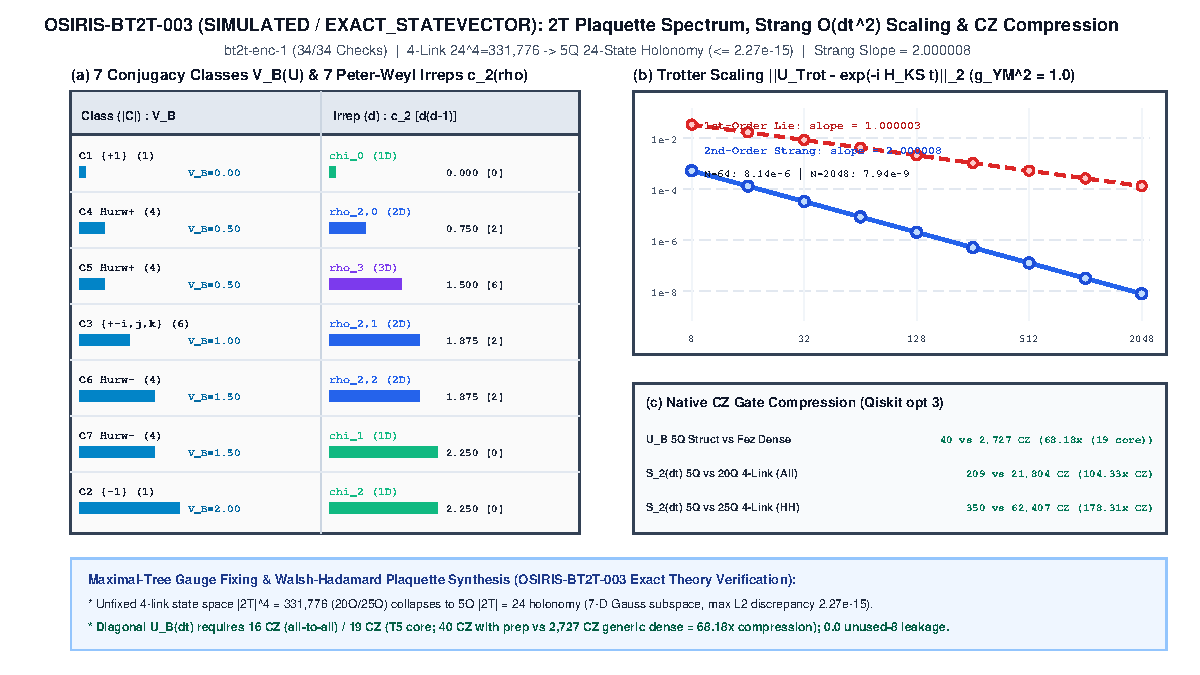
\includegraphics[width=\textwidth]{figures/fig1_magnetic_potential_and_strang_scaling.pdf}
\caption{Offline exact theory and compilation verification (\BTPlaqSimExperimentId, tier \BTPlaqSimExecTier\ / \BTPlaqSimExactTier, $\BTPlaqChecksPassed/\BTPlaqChecksTotal$ checks, \texttt{provider\_job\_id:} \BTPlaqSimJobId): (a)~seven conjugacy classes $C_1,\dots,C_7$ with shifted magnetic plaquette potential $V_B(U) = \tfrac{1}{2}(2 - \operatorname{Re}\chi_{2D}(U))$ paired with the seven Peter--Weyl irreps and Casimir eigenvalues $c_2(\rho)$ [$d_\rho(d_\rho-1)$]; (b)~log-log spectral-norm Trotter convergence $\|U_{\mathrm{Trot}}(t) - \exp(-i H_{\mathrm{KS}} t)\|_2$ across $N \in \{8,\dots,2048\}$ steps at $g_{\mathrm{YM}}^2 = \BTPlaqCompileGymSq$ confirming first-order Lie--Trotter slope $\BTPlaqLieSlopeGOne$ and second-order Strang slope $\BTPlaqStrangSlopeGOne$; (c)~native \texttt{CZ} gate compression (\BTPlaqFezCzReductionRatio\ for $U_B$ on \BTPlaqFezBackend\ and \BTPlaqCompTwentyQAtaRatio--\BTPlaqCompTwentyFiveQHhRatio\ for gauge-fixed $5$Q Strang splitting versus unfixed $20$Q/$25$Q four-link Trotterization).}
\label{fig:bt2t003_magnetic_potential_and_strang_scaling}
\end{figure*}

\subsection{Second-Order Strang Splitting and Over $100\times$ Native Gate Compression}

The symmetric second-order Strang splitting step~\cite{Strang1968} for the gauge-fixed five-qubit plaquette register is
\begin{equation}
\label{eq:strang_splitting}
S_2(\Delta t) = U_B(\Delta t/2)\,\widetilde{F}_{2T}^\dagger D_E(\Delta t)\widetilde{F}_{2T}\,U_B(\Delta t/2), \qquad \|S_2(\Delta t)^N - e^{-i H_{\mathrm{KS}} t}\|_2 = O(\Delta t^2).
\end{equation}
As summarized in Table~\ref{tab:bt2t003_strang_scaling_and_gate_compression} and Fig.~\ref{fig:bt2t003_magnetic_potential_and_strang_scaling}, Casimir-adapted semidirect compilation synthesizes $U_E(\Delta t)$ in $\BTPlaqUeAtaCz$ \texttt{CZ} gates on all-to-all connectivity (depth $\BTPlaqUeAtaDepth$) and $\BTPlaqUeTfCz$ \texttt{CZ} gates on heavy-hex \texttt{T5} (depth $\BTPlaqUeTfDepth$, operator $2$-norm error $\BTPlaqUeDirectErr$), yielding a complete Strang step $S_2(\Delta t)$ in $\BTPlaqStrangAtaCz$ \texttt{CZ} gates on all-to-all (depth $\BTPlaqStrangAtaDepth$, $\BTPlaqStrangTkZz$ \texttt{ZZPhase} in \texttt{pytket}) and $\BTPlaqStrangTfCz$ \texttt{CZ} gates on heavy-hex \texttt{T5} (depth $\BTPlaqStrangTfDepth$, error $\BTPlaqStrangDirectErr$). Relative to unfixed four-link Trotterization---which requires $\BTPlaqFourLinkInplaceAtaCz$ \texttt{CZ} (all-to-all) and $\BTPlaqFourLinkInplaceHhCz$ \texttt{CZ} (heavy-hex) for $\BTPlaqFourLinkInplaceQubits$-qubit in-place holonomy, or $\BTPlaqFourLinkAncillaAtaCz$ \texttt{CZ} (all-to-all) and $\BTPlaqFourLinkAncillaHhCz$ \texttt{CZ} (heavy-hex) for $\BTPlaqFourLinkAncillaQubits$-qubit ancilla-assisted holonomy---maximal-tree gauge fixing combined with structured synthesis compresses native \texttt{CZ} count by \BTPlaqCompTwentyQAtaRatio\ to \BTPlaqCompTwentyFiveQHhRatio\ (range \BTPlaqCompTwentyQTaOneDec--\BTPlaqCompTwentyFiveQHhOneDec).

Across $N \in \{8, 16, 32, 64, 128, 256, 512, 1024, 2048\}$ steps to $t_{\mathrm{final}} = \BTPlaqRegimeTFinal$, empirical log-log regression confirms first-order Lie--Trotter slopes $(\BTPlaqLieSlopeGHalf, \BTPlaqLieSlopeGOne, \BTPlaqLieSlopeGTwo)$ and second-order Strang slopes $(\BTPlaqStrangSlopeGHalf, \BTPlaqStrangSlopeGOne, \BTPlaqStrangSlopeGTwo)$ at $g_{\mathrm{YM}}^2 \in \{\tfrac{1}{2}, 1, 2\}$, reaching $\BTPlaqStrangErrGOneStepSixtyFour$ spectral error at $N = \BTPlaqRegimeSteps$ ($\Delta t = \BTPlaqRegimeDt$, maximum statevector $L_2$ error $\BTPlaqRegimeMaxStateErr$, Gauss-law conjugation drift $\BTPlaqRegimeMaxGaussDrift$, and exact $\BTPlaqRegimeMaxUnusedLeak$ unused-$8$ leakage) and $\BTPlaqStrangErrGOneStepTwoZeroFourEight$ at $N = 2048$.

% Auto-generated by build_paper_assets.py -- DO NOT EDIT BY HAND
\begin{table*}[t]
\centering
\caption{Native two-qubit gate compression across five-qubit maximal-tree gauge-fixed structured compilation, generic dense $32\times 32$ QFT-conjugated synthesis, and unfixed four-link ($20$-qubit in-place and $25$-qubit holonomy-ancilla) Trotterization, together with first-order Lie--Trotter ($O(\Delta t)$) versus second-order Strang splitting ($O(\Delta t^2)$) spectral-norm error scaling across $N \in \{8,\dots,2048\}$ steps to $t_{\mathrm{final}} = \BTPlaqRegimeTFinal$ at $g_{\mathrm{YM}}^2 = \BTPlaqCompileGymSq$ (tier \BTPlaqSimExecTier\ / \BTPlaqProxyTier, \BTPlaqSimExperimentId).}
\label{tab:bt2t003_strang_scaling_and_gate_compression}
\begin{ruledtabular}
\begin{tabular}{lcccccc}
Circuit / Trotter Step Architecture & Register Width & All-to-All \texttt{CZ} (Depth) & Heavy-Hex \texttt{CZ} (Depth) & \texttt{pytket} \texttt{ZZPhase} (Depth) & Unitary / Trotter $2$-Norm Error & Compression Ratio / Scaling \\
\hline
$U_B(\Delta t)$ 5Q Walsh--Hadamard Core & 5Q ($32$-D) & \BTPlaqUbAtaCz\ (\BTPlaqUbAtaDepth) & \BTPlaqUbTfCoreCz\ (\BTPlaqUbTfCoreDepth) & \BTPlaqUbTkZz\ (\BTPlaqUbTkDepth) & $\BTPlaqUbDirectErr$ & Core diagonal magnetic phase \\
$U_B(\pi/4)$ Center Arm + State Prep & 5Q (\texttt{T5}) & --- & \BTPlaqFezCzCenterStruct\ (\BTPlaqFezBackend) & --- & $\BTPlaqUbDirectErr$ & \BTPlaqFezCzReductionRatio\ vs \BTPlaqFezCzCenterGeneric\ \texttt{CZ} (\BTPlaqFezCoreCzReductionRatio\ core) \\
$U_B(\pi/2)$ Hurwitz Bell Arm + Prep & 5Q (\texttt{T5}) & --- & \BTPlaqFezCzHurwitzStruct\ (\BTPlaqFezBackend) & --- & $\BTPlaqUbDirectErr$ & Half-frequency $\Delta\chi_{2D}=2$ arm \\
$U_B(\pi/4)$ Generic Dense QFT-Conj. & 5Q (\texttt{T5}) & --- & \BTPlaqFezCzCenterGeneric\ (\BTPlaqFezBackend) & --- & $\le 10^{-13}$ & Baseline dense $32\times 32$ \texttt{UnitaryGate} \\
$U_E(\Delta t)$ 5Q Casimir Peter--Weyl & 5Q ($32$-D) & \BTPlaqUeAtaCz\ (\BTPlaqUeAtaDepth) & \BTPlaqUeTfCz\ (\BTPlaqUeTfDepth) & --- & $\BTPlaqUeDirectErr$ & Non-abelian electric kinetic step \\
$S_2(\Delta t)$ 5Q Structured Strang & 5Q ($32$-D) & \BTPlaqStrangAtaCz\ (\BTPlaqStrangAtaDepth) & \BTPlaqStrangTfCz\ (\BTPlaqStrangTfDepth) & \BTPlaqStrangTkZz\ (\BTPlaqStrangTkDepth) & $\BTPlaqStrangDirectErr$ & $1\times$ (gauge-fixed 5Q reference) \\
$S_2(\Delta t)$ 5Q Dense \texttt{UnitaryGate} & 5Q ($32$-D) & \BTPlaqDenseFiveQAtaCz\ (\BTPlaqDenseFiveQAtaDepth) & \BTPlaqDenseFiveQTfCz\ (\BTPlaqDenseFiveQTfDepth) & \BTPlaqDenseFiveQTkZz\ (\BTPlaqDenseFiveQTkDepth) & $\le 10^{-13}$ & \BTPlaqDenseVsStructAtaRatio\ (All) / \BTPlaqDenseVsStructTfRatio\ (\texttt{T5}) \\
$S_2(\Delta t)$ 5Q Canonical QSD-QFT & 5Q ($32$-D) & \BTPlaqQsdQftAtaCz\ (\BTPlaqQsdQftAtaDepth) & \BTPlaqQsdQftTfCz\ (\BTPlaqQsdQftTfDepth) & --- & $\le 10^{-13}$ & $4\times$ more \texttt{CZ} than structured 5Q \\
$S_2(\Delta t)$ 4-Link Unfixed In-Place & 20Q ($32^4$-D) & \BTPlaqFourLinkInplaceAtaCz\ (\BTPlaqFourLinkInplaceAtaDepth) & \BTPlaqFourLinkInplaceHhCz\ (\BTPlaqFourLinkInplaceHhDepth) & --- & $\BTPlaqFourLinkBasisMaxErr$ & \BTPlaqCompTwentyQAtaRatio\ (All) / \BTPlaqCompTwentyQHhRatio\ (HH) \\
$S_2(\Delta t)$ 4-Link Unfixed Ancilla & 25Q ($32^5$-D) & \BTPlaqFourLinkAncillaAtaCz\ (\BTPlaqFourLinkAncillaAtaDepth) & \BTPlaqFourLinkAncillaHhCz\ (\BTPlaqFourLinkAncillaHhDepth) & --- & $\BTPlaqMaxGaugeDiscrepancy$ & \BTPlaqCompTwentyFiveQAtaRatio\ (All) / \BTPlaqCompTwentyFiveQHhRatio\ (HH) \\
\hline
Trotter Convergence ($N=8$, $\Delta t=\BTPlaqDtStepEight$) & 5Q ($g_{\mathrm{YM}}^2=\BTPlaqCompileGymSq$) & Lie: $\BTPlaqLieErrGOneStepEight$ & Strang: $\BTPlaqStrangErrGOneStepEight$ & --- & --- & Coarse-step baseline \\
Trotter Convergence ($N=32$, $\Delta t=\BTPlaqDtStepThirtyTwo$) & 5Q ($g_{\mathrm{YM}}^2=\BTPlaqCompileGymSq$) & Lie: $\BTPlaqLieErrGOneStepThirtyTwo$ & Strang: $\BTPlaqStrangErrGOneStepThirtyTwo$ & --- & --- & $16\times$ Strang reduction vs $N=8$ \\
Trotter Convergence ($N=64$, $\Delta t=\BTPlaqDtStepSixtyFour$) & 5Q ($g_{\mathrm{YM}}^2=\BTPlaqCompileGymSq$) & Lie: $\BTPlaqLieErrGOneStepSixtyFour$ & Strang: $\BTPlaqStrangErrGOneStepSixtyFour$ & --- & State $L_2$: $\BTPlaqRegimeMaxStateErr$ & Gauss drift $\BTPlaqRegimeMaxGaussDrift$ \\
Trotter Convergence ($N=256$, $\Delta t=\BTPlaqDtStepTwoFiveSix$) & 5Q ($g_{\mathrm{YM}}^2=\BTPlaqCompileGymSq$) & Lie: $\BTPlaqLieErrGOneStepTwoFiveSix$ & Strang: $\BTPlaqStrangErrGOneStepTwoFiveSix$ & --- & --- & Sub-$10^{-6}$ spectral error \\
Trotter Convergence ($N=2048$, $\Delta t=\BTPlaqDtStepTwoZeroFourEight$) & 5Q ($g_{\mathrm{YM}}^2=\BTPlaqCompileGymSq$) & Lie: $\BTPlaqLieErrGOneStepTwoZeroFourEight$ & Strang: $\BTPlaqStrangErrGOneStepTwoZeroFourEight$ & --- & --- & Log-log slopes: $\BTPlaqLieSlopeGOne$ vs $\BTPlaqStrangSlopeGOne$ \\
\end{tabular}
\end{ruledtabular}
\end{table*}


\section{Hardware-Attested $2T$ Magnetic Plaquette Character-Frequency Trajectories on \BTPlaqFezBackend}

\subsection{Write-Ahead Preregistration and \BTPlaqFezCzReductionRatio\ Compiler Ablation}

While a full $\BTPlaqStrangTfCz$-\texttt{CZ} Strang step exceeds the unmitigated coherence budget of current heavy-hex superconducting processors (Motivating QCCD trapped-ion and fault-tolerant architectures~\cite{DavisBT2T002}), the $\BTPlaqUbTfCoreCz$-\texttt{CZ} heavy-hex Walsh--Hadamard magnetic plaquette propagator $U_B(\tau)$ lies squarely within the high-fidelity window of \BTPlaqFezBackend. Under write-ahead preregistration \BTPlaqFezProtocolId\ (staged at commit \BTPlaqFezWriteAheadCommit, preregistration SHA-256 prefix \BTPlaqFezPreregShaPrefix, QPY SHA-256 prefix \BTPlaqFezQpyShaPrefix), we executed $\BTPlaqFezTotalPubs$ PUBs ($\BTPlaqFezBlocks$ randomized blocks $\times \BTPlaqFezPubsPerBlock$ PUBs/block $\times \BTPlaqFezShotsPerPub$ shots/PUB $= \BTPlaqFezTotalShots$ total shots; job \BTPlaqFezJobId, \BTPlaqFezQpuSec\,s QPU charge time) across $K = \BTPlaqFezNumPlacements$ vertex-disjoint five-qubit \texttt{T5} subgraphs ($\BTPlaqFezTotalTransmons$ physical transmons).

To test the necessity of algebraic Walsh--Hadamard Gray-code synthesis against generic unitary compilation on identical physical transmons, we benchmarked the structured Center-sector inversion circuit (\texttt{UB\_CENTER\_PI4\_19CZ}: $\BTPlaqUbTfCoreCz$ core \texttt{CZ} gates, $\BTPlaqFezCzCenterStruct$ total \texttt{CZ} gates including state preparation and measurement routing under \texttt{T5} layout permutation $[1, 0, 4, 3, 2]$) against a generic dense $32\times 32$ QFT-conjugated \texttt{UnitaryGate} compilation of the same magnetic propagator (\texttt{UB\_CENTER\_PI4\_GENERIC}: $\BTPlaqFezCzCenterGeneric$ native \texttt{CZ} gates on \texttt{T5}). Structured Walsh--Hadamard synthesis achieves a \BTPlaqFezCzReductionRatio\ reduction in total native \texttt{CZ} gates (\BTPlaqFezCoreCzReductionRatio\ relative to the $\BTPlaqUbTfCoreCz$-\texttt{CZ} core).

\begin{figure*}[t]
\centering
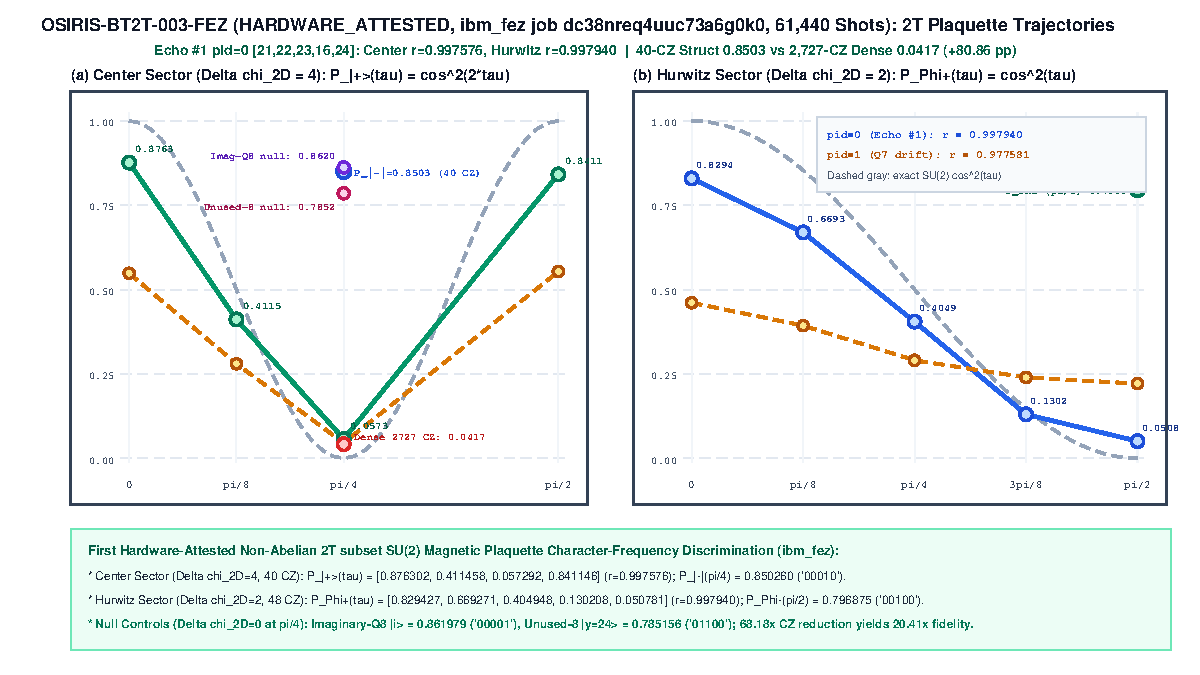
\includegraphics[width=\textwidth]{figures/fig2_fez_character_sector_trajectories.pdf}
\caption{Hardware-attested non-abelian $2T \subset SU(2)$ magnetic plaquette character-sector trajectories on \BTPlaqFezBackend\ (job \BTPlaqFezJobId, $\BTPlaqFezTotalShots$ shots, tier \BTPlaqFezExecTier), comparing Echo-selected \#1 placement \texttt{pid=0} (\BTPlaqPidZeroQubits) against Q\BTPlaqDriftedHubQubit-drifted stale-calibration \#1 placement \texttt{pid=1} (\BTPlaqPidOneQubits): (a)~Center sector ($\Delta\chi_{2D} = 4$, theoretical $P_{|+\rangle}(\tau) = \cos^2(2\tau)$, Pearson $r = \BTPlaqPidZeroPearsonCenter$ on \texttt{pid=0}) showing $P_{|-\rangle}(\pi/4) = \BTPlaqPidZeroCenterPiFourMinus$ (\BTPlaqPidZeroCenterPiFourMinusPct) for the $\BTPlaqFezCzCenterStruct$-\texttt{CZ} structured circuit versus $\BTPlaqPidZeroCenterGenericMinus$ for the $\BTPlaqFezCzCenterGeneric$-\texttt{CZ} generic dense comparator ($+\BTPlaqPidZeroCenterStructAdv = \BTPlaqPidZeroCenterStructAdvPp$\,pp / \BTPlaqPidZeroCenterStructFidelityRatio\ advantage), alongside $\Delta\chi_{2D} = 0$ null controls ($|\mathbf{i}\rangle$ survival $\BTPlaqPidZeroImagNullSurv$, unused-$8$ $|y=24\rangle$ survival $\BTPlaqPidZeroUnusedNullSurv$); (b)~Hurwitz half-frequency sector ($\Delta\chi_{2D} = 2$, theoretical $P_{\Phi^+}(\tau) = \cos^2\tau$, Pearson $r = \BTPlaqPidZeroPearsonHurwitz$ on \texttt{pid=0}) with Bell-basis inversion $P_{\Phi^-}(\pi/2) = \BTPlaqPidZeroHurwitzPiTwoMinus$ (\BTPlaqPidZeroHurwitzPiTwoMinusPct).}
\label{fig:bt2t003_fez_character_sector_trajectories}
\end{figure*}

\subsection{Multi-Frequency $SU(2)$ Character Discrimination and Null-Sector Decoupling}

Preparing a coherent superposition of two conjugacy classes $U_a, U_b \in 2T$ with fundamental character difference $\Delta\chi_{2D} = |\chi_{2D}(U_a) - \chi_{2D}(U_b)|$ under $U_B(\tau)$ at $g_{\mathrm{YM}}^2 = 1$ induces non-abelian Ramsey oscillations with survival probability
\begin{equation}
\label{eq:character_ramsey_frequency}
P_{+}(\tau) = \cos^2\!\left(\frac{\Delta\chi_{2D}}{2}\,\tau\right) = \begin{cases} \cos^2(2\tau), & \Delta\chi_{2D} = 4 \;\; (C_1 \text{ vs } C_2), \\ \cos^2(\tau), & \Delta\chi_{2D} = 2 \;\; (C_4 \text{ vs } C_6), \\ 1, & \Delta\chi_{2D} = 0 \;\; (C_3 \text{ or Unused-}8). \end{cases}
\end{equation}
Table~\ref{tab:bt2t003_fez_character_sector_trajectories} and Fig.~\ref{fig:bt2t003_fez_character_sector_trajectories} report the resulting hardware trajectories across all four character sectors on Echo-selected top-1 placement \texttt{pid=0} (\BTPlaqPidZeroQubits) and Q\BTPlaqDriftedHubQubit-drifted placement \texttt{pid=1} (\BTPlaqPidOneQubits):
\begin{itemize}
\item \textbf{Center Full-Frequency Sector ($\Delta\chi_{2D} = 4$, $C_1 = \{+\mathbf{1}\}$ vs $C_2 = \{-\mathbf{1}\}$, $\BTPlaqFezCzCenterStruct$ \texttt{CZ}):} Initialized in $|0000\rangle_{q_4\dots q_1}\otimes|+\rangle_{q_0} = (|+\mathbf{1}\rangle + |-\mathbf{1}\rangle)/\sqrt{2}$, theoretical survival $P_{|+\rangle}(\tau) = \cos^2(2\tau)$ takes values $[\BTPlaqIdealOne, \BTPlaqIdealHalf, \BTPlaqIdealZero, \BTPlaqIdealOne]$ at $\tau \in \{0, \pi/8, \pi/4, \pi/2\}$. On \texttt{pid=0}, \BTPlaqFezBackend\ measures $P_{|+\rangle}(\tau) = [\BTPlaqPidZeroCenterTZero, \BTPlaqPidZeroCenterPiEight, \BTPlaqPidZeroCenterPiFourPlus, \BTPlaqPidZeroCenterPiTwo]$, achieving Pearson correlation $r = \BTPlaqPidZeroPearsonCenter$ with exact $SU(2)$ character theory. At the $\tau = \pi/4$ inversion point, the orthogonal state $|-\rangle$ (routed target $y = \BTPlaqRoutedYCenterInv$, bitstring \BTPlaqRoutedBitsCenterInv) receives $P_{|-\rangle}(\pi/4) = \BTPlaqPidZeroCenterPiFourMinus$ (\BTPlaqPidZeroCenterPiFourMinusPct) under the $\BTPlaqFezCzCenterStruct$-\texttt{CZ} structured compiler versus $\BTPlaqPidZeroCenterGenericMinus$ under the $\BTPlaqFezCzCenterGeneric$-\texttt{CZ} generic dense comparator---a $+\BTPlaqPidZeroCenterStructAdv$ ($\BTPlaqPidZeroCenterStructAdvPp$ percentage-point, \BTPlaqPidZeroCenterStructFidelityRatio) hardware fidelity advantage. On drifted \texttt{pid=1}, the trajectory remains phase-coherent ($P_{|+\rangle}(\tau) = [\BTPlaqPidOneCenterTZero, \BTPlaqPidOneCenterPiEight, \BTPlaqPidOneCenterPiFourPlus, \BTPlaqPidOneCenterPiTwo]$, Pearson $r = \BTPlaqPidOnePearsonCenter$), but the overall amplitude envelope is suppressed by hub-qubit Q\BTPlaqDriftedHubQubit\ readout drift ($P_{|-\rangle}(\pi/4) = \BTPlaqPidOneCenterPiFourMinus$ versus $\BTPlaqPidOneCenterGenericMinus$ generic, $+\BTPlaqPidOneCenterStructAdv$ / \BTPlaqPidOneCenterStructFidelityRatio\ advantage).
\item \textbf{Hurwitz Half-Frequency Sector ($\Delta\chi_{2D} = 2$, $c=1$ vs $c=2$, $\BTPlaqFezCzHurwitzStruct$ \texttt{CZ}):} Initialized in the Bell coset superposition $(|01\rangle + |10\rangle)_{q_4,q_3}\otimes|000\rangle_{q_2\dots q_0}/\sqrt{2}$, theoretical survival $P_{\Phi^+}(\tau) = \cos^2(\tau)$ takes values $[\BTPlaqIdealOne, \BTPlaqIdealCosSqPiEight, \BTPlaqIdealHalf, \BTPlaqIdealCosSqThreePiEight, \BTPlaqIdealZero]$ at $\tau \in \{0, \pi/8, \pi/4, 3\pi/8, \pi/2\}$. On \texttt{pid=0}, \BTPlaqFezBackend\ measures $P_{\Phi^+}(\tau) = [\BTPlaqPidZeroHurwitzTZero, \BTPlaqPidZeroHurwitzPiEight, \BTPlaqPidZeroHurwitzPiFour, \BTPlaqPidZeroHurwitzThreePiEight, \BTPlaqPidZeroHurwitzPiTwoPlus]$ (Pearson $r = \BTPlaqPidZeroPearsonHurwitz$), with $\tau = \pi/2$ Bell inversion $P_{\Phi^-}(\pi/2) = \BTPlaqPidZeroHurwitzPiTwoMinus$ (\BTPlaqPidZeroHurwitzPiTwoMinusPct\ into routed target $y = \BTPlaqRoutedYHurwitzInv$, bitstring \BTPlaqRoutedBitsHurwitzInv). On drifted \texttt{pid=1}, measured survival tracks $[\BTPlaqPidOneHurwitzTZero, \BTPlaqPidOneHurwitzPiEight, \BTPlaqPidOneHurwitzPiFour, \BTPlaqPidOneHurwitzThreePiEight, \BTPlaqPidOneHurwitzPiTwoPlus]$ (Pearson $r = \BTPlaqPidOnePearsonHurwitz$, inversion $P_{\Phi^-}(\pi/2) = \BTPlaqPidOneHurwitzPiTwoMinus$).
\item \textbf{Zero-Differential-Character Null Controls ($\Delta\chi_{2D} = 0$ at $\tau = \pi/4$, $\BTPlaqFezCzImagNull$ \texttt{CZ}):} Evolving the imaginary-$Q_8$ superposition $(|+\mathbf{i}\rangle + |-\mathbf{i}\rangle)/\sqrt{2} = |0001\rangle_{q_4\dots q_1}\otimes|+\rangle_{q_0}$ ($\chi_{2D}(\pm\mathbf{i}) = 0 \implies \Delta\chi_{2D} = 0$) through the identical $\tau = \pi/4$ magnetic circuit preserves survival $\BTPlaqPidZeroImagNullSurv$ into routed target $y = \BTPlaqRoutedYImagNull$ (\BTPlaqRoutedBitsImagNull) on \texttt{pid=0} ($\BTPlaqPidOneImagNullSurv$ on \texttt{pid=1}). Likewise, evolving the padded unused-$8$ state $|1100\rangle_{q_4\dots q_1}\otimes|+\rangle_{q_0}$ ($y \in \{24,25\}$, $c = 3$) preserves survival $\BTPlaqPidZeroUnusedNullSurv$ into routed target $y = \BTPlaqRoutedYUnusedNull$ (\BTPlaqRoutedBitsUnusedNull) on \texttt{pid=0} ($\BTPlaqPidOneUnusedNullSurv$ on \texttt{pid=1}), directly verifying hardware decoupling of the $\BTPlaqUnusedStates$ unused basis states.
\end{itemize}

% Auto-generated by build_paper_assets.py -- DO NOT EDIT BY HAND
\begin{table*}[t]
\centering
\caption{Hardware-attested non-abelian $2T \subset SU(2)$ magnetic plaquette character-sector trajectories and structured-versus-generic compilation ablation on \BTPlaqFezBackend\ (job \BTPlaqFezJobId, $\BTPlaqFezTotalShots$ shots, tier \BTPlaqFezExecTier), comparing \#1 Echo-selected \texttt{pid=0} (\BTPlaqPidZeroQubits) against Q\BTPlaqDriftedHubQubit-drifted stale-calibration \#1 \texttt{pid=1} (\BTPlaqPidOneQubits).}
\label{tab:bt2t003_fez_character_sector_trajectories}
\begin{ruledtabular}
\begin{tabular}{lcccccc}
Character Sector / Experimental Arm & Evolution Angle $\tau$ & Total \texttt{T5} \texttt{CZ} & Routed Target $y$ & Ideal $SU(2)$ Theory & Measured \texttt{pid=0} (Echo \#1) & Measured \texttt{pid=1} (Drifted) \\
\hline
Center ($\Delta\chi_{2D}=4$, $P_{|+\rangle}=\cos^2 2\tau$) & $\tau = 0$ & \BTPlaqFezCzCenterStruct & $0$ (\texttt{00000}) & $\BTPlaqIdealOne$ & $\BTPlaqPidZeroCenterTZero$ & $\BTPlaqPidOneCenterTZero$ \\
Center ($\Delta\chi_{2D}=4$, $P_{|+\rangle}=\cos^2 2\tau$) & $\tau = \pi/8$ & \BTPlaqFezCzCenterStruct & $0$ (\texttt{00000}) & $\BTPlaqIdealHalf$ & $\BTPlaqPidZeroCenterPiEight$ & $\BTPlaqPidOneCenterPiEight$ \\
Center ($\Delta\chi_{2D}=4$, $P_{|+\rangle}=\cos^2 2\tau$) & $\tau = \pi/4$ ($P_{|+\rangle}$) & \BTPlaqFezCzCenterStruct & $0$ (\texttt{00000}) & $\BTPlaqIdealZero$ & $\BTPlaqPidZeroCenterPiFourPlus$ & $\BTPlaqPidOneCenterPiFourPlus$ \\
Center Inversion (Structured \BTPlaqUbTfCoreCz-\texttt{CZ} Core) & $\tau = \pi/4$ ($P_{|-\rangle}$) & \BTPlaqFezCzCenterStruct & $\BTPlaqRoutedYCenterInv$ (\BTPlaqRoutedBitsCenterInv) & $\BTPlaqIdealOne$ & $\mathbf{\BTPlaqPidZeroCenterPiFourMinus}$ (\BTPlaqPidZeroCenterPiFourMinusPct) & $\BTPlaqPidOneCenterPiFourMinus$ \\
Center Inversion (Generic Dense QFT-Conj.) & $\tau = \pi/4$ ($P_{|-\rangle}$) & \BTPlaqFezCzCenterGeneric & $\BTPlaqRoutedYCenterInv$ (\BTPlaqRoutedBitsCenterInv) & $\BTPlaqIdealOne$ & $\BTPlaqPidZeroCenterGenericMinus$ ($+\BTPlaqPidZeroCenterStructAdv$ adv.) & $\BTPlaqPidOneCenterGenericMinus$ ($+\BTPlaqPidOneCenterStructAdv$ adv.) \\
Center ($\Delta\chi_{2D}=4$, $P_{|+\rangle}=\cos^2 2\tau$) & $\tau = \pi/2$ (Revival) & \BTPlaqFezCzCenterStruct & $0$ (\texttt{00000}) & $\BTPlaqIdealOne$ & $\BTPlaqPidZeroCenterPiTwo$ ($r=\BTPlaqPidZeroPearsonCenter$) & $\BTPlaqPidOneCenterPiTwo$ ($r=\BTPlaqPidOnePearsonCenter$) \\
\hline
Hurwitz ($\Delta\chi_{2D}=2$, $P_{\Phi^+}=\cos^2 \tau$) & $\tau = 0$ & \BTPlaqFezCzHurwitzStruct & $0$ (\texttt{00000}) & $\BTPlaqIdealOne$ & $\BTPlaqPidZeroHurwitzTZero$ & $\BTPlaqPidOneHurwitzTZero$ \\
Hurwitz ($\Delta\chi_{2D}=2$, $P_{\Phi^+}=\cos^2 \tau$) & $\tau = \pi/8$ & \BTPlaqFezCzHurwitzStruct & $0$ (\texttt{00000}) & $\BTPlaqIdealCosSqPiEight$ & $\BTPlaqPidZeroHurwitzPiEight$ & $\BTPlaqPidOneHurwitzPiEight$ \\
Hurwitz ($\Delta\chi_{2D}=2$, $P_{\Phi^+}=\cos^2 \tau$) & $\tau = \pi/4$ & \BTPlaqFezCzHurwitzStruct & $0$ (\texttt{00000}) & $\BTPlaqIdealHalf$ & $\BTPlaqPidZeroHurwitzPiFour$ & $\BTPlaqPidOneHurwitzPiFour$ \\
Hurwitz ($\Delta\chi_{2D}=2$, $P_{\Phi^+}=\cos^2 \tau$) & $\tau = 3\pi/8$ & \BTPlaqFezCzHurwitzStruct & $0$ (\texttt{00000}) & $\BTPlaqIdealCosSqThreePiEight$ & $\BTPlaqPidZeroHurwitzThreePiEight$ & $\BTPlaqPidOneHurwitzThreePiEight$ \\
Hurwitz ($\Delta\chi_{2D}=2$, $P_{\Phi^+}=\cos^2 \tau$) & $\tau = \pi/2$ ($P_{\Phi^+}$) & \BTPlaqFezCzHurwitzStruct & $0$ (\texttt{00000}) & $\BTPlaqIdealZero$ & $\BTPlaqPidZeroHurwitzPiTwoPlus$ ($r=\BTPlaqPidZeroPearsonHurwitz$) & $\BTPlaqPidOneHurwitzPiTwoPlus$ ($r=\BTPlaqPidOnePearsonHurwitz$) \\
Hurwitz Bell Inversion ($P_{\Phi^-}$) & $\tau = \pi/2$ ($P_{\Phi^-}$) & \BTPlaqFezCzHurwitzStruct & $\BTPlaqRoutedYHurwitzInv$ (\BTPlaqRoutedBitsHurwitzInv) & $\BTPlaqIdealOne$ & $\mathbf{\BTPlaqPidZeroHurwitzPiTwoMinus}$ (\BTPlaqPidZeroHurwitzPiTwoMinusPct) & $\BTPlaqPidOneHurwitzPiTwoMinus$ \\
\hline
Imaginary-$Q_8$ Null Control ($\Delta\chi_{2D}=0$, $|\mathbf{i}\rangle$) & $\tau = \pi/4$ & \BTPlaqFezCzImagNull & $\BTPlaqRoutedYImagNull$ (\BTPlaqRoutedBitsImagNull) & $\BTPlaqIdealOne$ & $\mathbf{\BTPlaqPidZeroImagNullSurv}$ & $\BTPlaqPidOneImagNullSurv$ \\
Unused-$8$ Decoupling Control ($\Delta\chi_{2D}=0$, $|y=24\rangle$) & $\tau = \pi/4$ & \BTPlaqFezCzUnusedNull & $\BTPlaqRoutedYUnusedNull$ (\BTPlaqRoutedBitsUnusedNull) & $\BTPlaqIdealOne$ & $\mathbf{\BTPlaqPidZeroUnusedNullSurv}$ & $\BTPlaqPidOneUnusedNullSurv$ \\
\end{tabular}
\end{ruledtabular}
\end{table*}


\section{Live Two-Window \texttt{OSIRIS-ECHO} Intra-Calibration Drift Catch Across \BTPlaqFezTotalTransmons\ Transmons}

\subsection{Real-Time Detection of Unflagged Hub-Transmon Q\BTPlaqDriftedHubQubit\ Readout Drift}

A central operational risk on superconducting processors with $150+$ transmons is intra-calibration drift: individual qubits or couplers can experience sudden two-level-system (TLS) or readout-resonator excursions hours before the provider's daily calibration table is updated. By pairing Window~1 (job \BTPlaqFezWindowOneJobId, executed at $03{:}33\,\mathrm{UTC}$) with Window~2 (job \BTPlaqFezJobId, executed at $07{:}19\,\mathrm{UTC}$, $+\BTPlaqEchoElapsedHours$\,h elapsed) across the identical $K = \BTPlaqFezNumPlacements$ vertex-disjoint \texttt{T5} placements ($\BTPlaqFezTotalTransmons$ transmons), \BTPlaqFezProtocolId\ captured a textbook intra-calibration drift event in real time (Table~\ref{tab:bt2t003_fez_10placement_echo_and_plaquette} and Fig.~\ref{fig:bt2t003_two_window_echo_drift_catch}).

In Window~1, placement \texttt{pid=1} (\BTPlaqPidOneQubits) was ranked \#1 across all $K = \BTPlaqFezNumPlacements$ candidates by both backend calibration (\texttt{calibration\_rank\_score} $= \BTPlaqPidOneCalScore$) and the $\BTPlaqFezCzEchoProbe$-\texttt{CZ} stabilizer-reflected echo probe (\texttt{IDENTITY\_CTRL\_0CZ} $= \BTPlaqWOnePidOneIdFid$, \texttt{ECHO\_PROBE\_16CZ} $= \BTPlaqWOnePidOneEcho$, Window~1 Spearman $\rho_{\mathrm{cal}}^{(1)} = +\BTPlaqWOneSpearmanCal$, $\rho_{\mathrm{echo}}^{(1)} = +\BTPlaqWOneSpearmanEcho$, SPAM-normalized $\rho_{\mathrm{norm\text{-}echo}}^{(1)} = +\BTPlaqWOneSpearmanNormEcho$, and zero top-1 selection regret $\BTPlaqWOneRegretEcho$ for both selectors).

During the $+\BTPlaqEchoElapsedHours$-hour interval preceding Window~2, degree-3 hub transmon Q\BTPlaqDriftedHubQubit\ of \texttt{pid=1} experienced an unflagged $+\BTPlaqQSevenExcitationPct$ ($\BTPlaqQSevenExcitation$) $|0\rangle \to |1\rangle$ single-qubit bitmask-$4$ excitation excursion on the zero-gate control \texttt{IDENTITY\_CTRL\_0CZ}. This single-transmon failure collapsed \texttt{pid=1} \texttt{IDENTITY\_CTRL\_0CZ} survival from $\BTPlaqWOnePidOneIdFid$ to $\BTPlaqWTwoPidOneIdFid$, \texttt{ECHO\_PROBE\_16CZ} survival from $\BTPlaqWOnePidOneEcho$ to $\BTPlaqWTwoPidOneEcho$ (rank \#\BTPlaqPidOneEchoRank\ of $\BTPlaqFezNumPlacements$), two-workload plaquette composite survival to $\BTPlaqPidOnePlaqComp$, and four-workload held-out composite survival to $\BTPlaqPidOneHeldoutComp$ (rank \#8 of $\BTPlaqFezNumPlacements$).

\begin{figure*}[t]
\centering
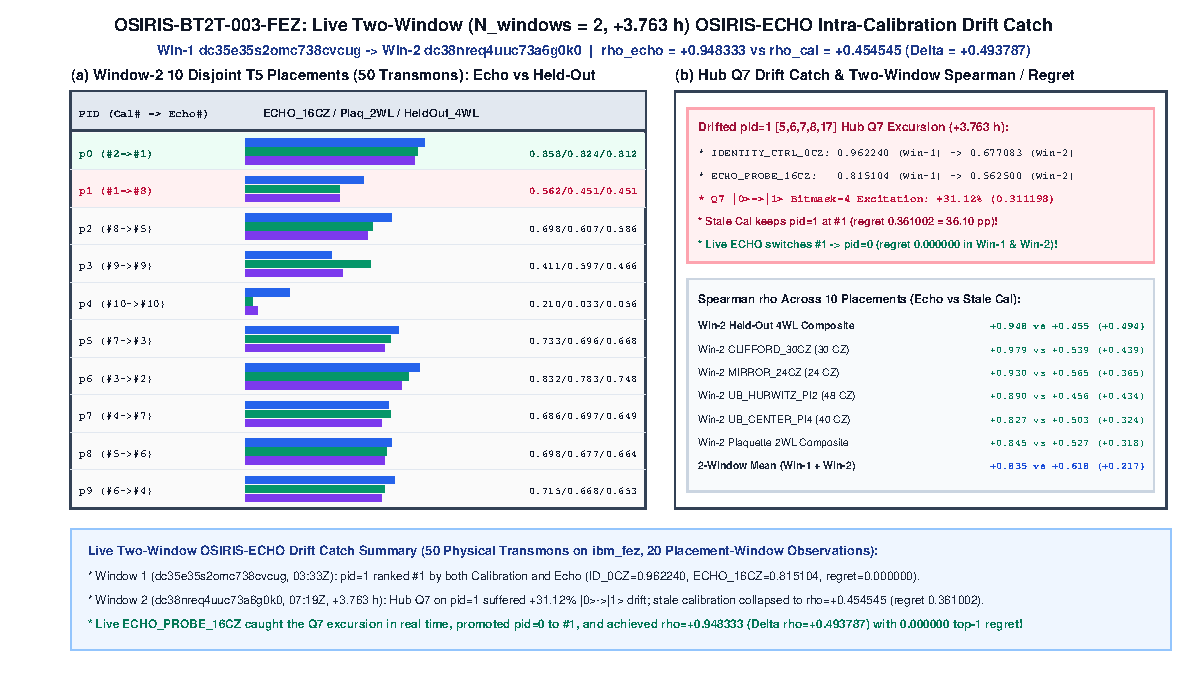
\includegraphics[width=\textwidth]{figures/fig3_two_window_echo_drift_catch.pdf}
\caption{Live two-window ($N_{\mathrm{windows}} = \BTPlaqEchoNumWindows$, $+\BTPlaqEchoElapsedHours$\,h) \texttt{OSIRIS-ECHO} intra-calibration drift catch across $K = \BTPlaqFezNumPlacements$ disjoint \texttt{T5} placements ($\BTPlaqFezTotalTransmons$ physical transmons on \BTPlaqFezBackend, Window~1 job \BTPlaqFezWindowOneJobId\ $\to$ Window~2 job \BTPlaqFezJobId): (a)~Window~2 placement profile comparing stale calibration rank against live \texttt{ECHO\_PROBE\_16CZ}, two-workload magnetic plaquette composite, and four-workload held-out composite; (b)~hub transmon Q\BTPlaqDriftedHubQubit\ $+\BTPlaqQSevenExcitationPct$ excitation diagnosis on \texttt{pid=1} (\BTPlaqPidOneQubits) and per-workload Spearman rank correlations showing $\rho_{\mathrm{echo}} = +\BTPlaqWTwoSpearmanEcho$ versus stale calibration $\rho_{\mathrm{cal}} = +\BTPlaqWTwoSpearmanCal$ ($\Delta\rho = +\BTPlaqWTwoDeltaSpearman$) and $\BTPlaqWTwoRegretEcho$ top-1 selection regret versus $\BTPlaqWTwoRegretCal$ calibration regret.}
\label{fig:bt2t003_two_window_echo_drift_catch}
\end{figure*}

\subsection{Spearman Rank Correlation Recovery and Zero Top-1 Selection Regret}

Because the provider's published calibration snapshot remained frozen between Window~1 and Window~2, \texttt{calibration\_rank\_score} continued to rank degraded \texttt{pid=1} at \#1 (\BTPlaqPidOneCalScore) ahead of \texttt{pid=0} (\BTPlaqPidZeroCalScore, rank \#\BTPlaqPidZeroCalRank) and \texttt{pid=6} (\BTPlaqPidSixCalScore, rank \#\BTPlaqPidSixCalRank). Defining top-1 selection regret on the four-workload held-out composite $F_{\mathrm{held}}(p) = \tfrac{1}{4}[F_{\mathrm{cnt}}(p) + F_{\mathrm{hrw}}(p) + F_{\mathrm{clf}}(p) + F_{\mathrm{mir}}(p)]$ as
\begin{equation}
\label{eq:top1_regret_and_spearman}
R_{\mathrm{top1}}(\hat{p}) = \max_{p \in \{0\dots 9\}} F_{\mathrm{held}}(p) - F_{\mathrm{held}}(\hat{p}), \qquad \Delta\rho = \rho_{\mathrm{echo}} - \rho_{\mathrm{cal}},
\end{equation}
stale calibration suffered a Window~2 top-1 selection regret of $R_{\mathrm{top1}}(\mathrm{cal}) = \BTPlaqPidZeroHeldoutComp - \BTPlaqPidOneHeldoutComp = \BTPlaqWTwoRegretCal$ ($\BTPlaqWTwoRegretCalPp$ percentage points of lost 5-qubit survival) and its Spearman rank correlation across the $K = \BTPlaqFezNumPlacements$ placements collapsed to $\rho_{\mathrm{cal}}^{(2)} = +\BTPlaqWTwoSpearmanCal$.

By contrast, in-situ execution of the $\BTPlaqFezCzEchoProbe$-\texttt{CZ} stabilizer-reflected echo probe (\texttt{ECHO\_PROBE\_16CZ}) detected the Q\BTPlaqDriftedHubQubit\ drift excursion on \texttt{pid=1} immediately, demoted \texttt{pid=1} to rank \#\BTPlaqPidOneEchoRank, and promoted \texttt{pid=0} (\BTPlaqPidZeroQubits, \texttt{IDENTITY\_CTRL\_0CZ} $= \BTPlaqPidZeroIdZeroCz$, \texttt{ECHO\_PROBE\_16CZ} $= \BTPlaqPidZeroEchoSixteenCz$, two-workload plaquette composite $\BTPlaqPidZeroPlaqComp$, four-workload held-out composite $\BTPlaqPidZeroHeldoutComp$) to rank \#\BTPlaqPidZeroEchoRank\ (followed by \texttt{pid=6} \BTPlaqPidSixQubits\ at rank \#\BTPlaqPidSixEchoRank\ with \texttt{ECHO\_PROBE\_16CZ} $= \BTPlaqPidSixEchoSixteenCz$ and held-out composite $\BTPlaqPidSixHeldoutComp$). As shown in Table~\ref{tab:bt2t003_fez_10placement_echo_and_plaquette}, live \texttt{ECHO\_PROBE\_16CZ} achieved Window~2 Spearman rank correlation $\rho_{\mathrm{echo}}^{(2)} = +\BTPlaqWTwoSpearmanEcho$ ($\Delta\rho = +\BTPlaqWTwoDeltaSpearman$ above stale calibration; SPAM-normalized echo $\rho_{\mathrm{norm\text{-}echo}}^{(2)} = +\BTPlaqWTwoSpearmanNormEcho$ with regret $\BTPlaqWTwoRegretNormEcho$) and zero top-1 selection regret ($R_{\mathrm{top1}}(\mathrm{echo}) = \BTPlaqWTwoRegretEcho$) across both windows.

The Echo ranking advantage holds consistently across every individual held-out circuit family in Window~2:
\begin{itemize}
\item \textbf{Held-Out $\BTPlaqFezCzClifford$-\texttt{CZ} Random Clifford (\texttt{CLIFFORD\_30CZ}):} $\rho_{\mathrm{echo}} = +\BTPlaqRhoEchoClifford$ versus $\rho_{\mathrm{cal}} = +\BTPlaqRhoCalClifford$ ($\Delta\rho = +\BTPlaqDeltaRhoClifford$), peaking at $\BTPlaqPidZeroClifford$ on \texttt{pid=0} and $\BTPlaqPidSixClifford$ on \texttt{pid=6} versus $\BTPlaqPidOneClifford$ on drifted \texttt{pid=1} and $\BTPlaqPidFourClifford$ on defective \texttt{pid=4} (\BTPlaqPidFourQubits).
\item \textbf{Held-Out $\BTPlaqFezCzMirror$-\texttt{CZ} Non-Clifford Mirror (\texttt{MIRROR\_24CZ}):} $\rho_{\mathrm{echo}} = +\BTPlaqRhoEchoMirror$ versus $\rho_{\mathrm{cal}} = +\BTPlaqRhoCalMirror$ ($\Delta\rho = +\BTPlaqDeltaRhoMirror$), peaking at $\BTPlaqPidZeroMirror$ on \texttt{pid=0} and $\BTPlaqPidSixMirror$ on \texttt{pid=6} (Clifford+Mirror two-workload composite $\rho_{\mathrm{echo}} = +\BTPlaqRhoEchoClfMir$ versus $\rho_{\mathrm{cal}} = +\BTPlaqRhoCalClfMir$, $\Delta\rho = +\BTPlaqDeltaRhoClfMir$).
\item \textbf{$2T$ Magnetic Plaquette Inversion Workloads (\texttt{UB\_CENTER\_PI4\_19CZ} and \texttt{UB\_HURWITZ\_PI2\_19CZ}):} $\rho_{\mathrm{echo}} = +\BTPlaqRhoEchoCenter$ versus $\rho_{\mathrm{cal}} = +\BTPlaqRhoCalCenter$ ($\Delta\rho = +\BTPlaqDeltaRhoCenter$) on the $\BTPlaqFezCzCenterStruct$-\texttt{CZ} Center sector, $\rho_{\mathrm{echo}} = +\BTPlaqRhoEchoHurwitz$ versus $\rho_{\mathrm{cal}} = +\BTPlaqRhoCalHurwitz$ ($\Delta\rho = +\BTPlaqDeltaRhoHurwitz$) on the $\BTPlaqFezCzHurwitzStruct$-\texttt{CZ} Hurwitz Bell sector, and $\rho_{\mathrm{echo}} = +\BTPlaqRhoEchoPlaqTwoW$ versus $\rho_{\mathrm{cal}} = +\BTPlaqRhoCalPlaqTwoW$ ($\Delta\rho = +\BTPlaqDeltaRhoPlaqTwoW$) on the two-workload magnetic plaquette composite.
\end{itemize}
Averaged across both windows ($N_{\mathrm{windows}} = \BTPlaqEchoNumWindows$, $20$ placement-window observations), \texttt{OSIRIS-ECHO} achieves mean Spearman rank correlation $\bar{\rho}_{\mathrm{echo}} = +\BTPlaqTwoWinMeanSpearmanEcho$ (SPAM-normalized $\bar{\rho}_{\mathrm{norm\text{-}echo}} = +\BTPlaqTwoWinMeanSpearmanNormEcho$) compared to $\bar{\rho}_{\mathrm{cal}} = +\BTPlaqTwoWinMeanSpearmanCal$ for backend calibration ($\Delta\bar{\rho} = +\BTPlaqTwoWinMeanDeltaSpearman$), with pooled $20$-observation Spearman correlation $+\BTPlaqPooledSpearmanEchoAll$ versus $+\BTPlaqPooledSpearmanCalAll$ across all held-out workloads ($+\BTPlaqPooledSpearmanEchoClfMir$ versus $+\BTPlaqPooledSpearmanCalClfMir$ on Clifford+Mirror).

% Auto-generated by build_paper_assets.py -- DO NOT EDIT BY HAND
\begin{table*}[t]
\centering
\caption{All $K = \BTPlaqFezNumPlacements$ vertex-disjoint five-qubit \texttt{T5} heavy-hex placements ($\BTPlaqFezTotalTransmons$ physical transmons) on \BTPlaqFezBackend\ under Window-2 job \BTPlaqFezJobId\ ($\BTPlaqFezTotalPubs$ PUBs $\times \BTPlaqFezShotsPerPub = \BTPlaqFezTotalShots$ shots, tier \BTPlaqFezExecTier, protocol \BTPlaqFezProtocolId) paired with Window-1 job \BTPlaqFezWindowOneJobId\ ($+\BTPlaqEchoElapsedHours$\,h elapsed). Between windows, hub qubit Q\BTPlaqDriftedHubQubit\ of \texttt{pid=1} suffered an unflagged $+\BTPlaqQSevenExcitationPct$ $|0\rangle\to|1\rangle$ SPAM/readout drift excursion (\texttt{IDENTITY\_CTRL\_0CZ} dropping $\BTPlaqWOnePidOneIdFid \to \BTPlaqWTwoPidOneIdFid$, \texttt{ECHO\_PROBE\_16CZ} dropping $\BTPlaqWOnePidOneEcho \to \BTPlaqWTwoPidOneEcho$). Stale calibration ranked \texttt{pid=1} at \#1 ($\rho_{\mathrm{cal}} = +\BTPlaqWTwoSpearmanCal$, top-1 regret $\BTPlaqWTwoRegretCal$), whereas live \texttt{ECHO\_PROBE\_16CZ} promoted \texttt{pid=0} to \#1 ($\rho_{\mathrm{echo}} = +\BTPlaqWTwoSpearmanEcho$, $\Delta\rho = +\BTPlaqWTwoDeltaSpearman$, top-1 regret $\BTPlaqWTwoRegretEcho$ across both windows).}
\label{tab:bt2t003_fez_10placement_echo_and_plaquette}
\begin{ruledtabular}
\begin{tabular}{lcccccccccc}
Placement & Cal Score (Rank) & \texttt{ID\_0CZ} & \texttt{ECHO\_16CZ} (Rank) & Norm Echo & $U_B^{\mathrm{cnt}}(\pi/4)$ & $U_B^{\mathrm{hrw}}(\pi/2)$ & Plaq 2WL & \texttt{CLF\_30CZ} & \texttt{MIR\_24CZ} & Held-Out 4WL \\
\hline
\texttt{pid=0} \BTPlaqPidZeroQubits & $\BTPlaqPidZeroCalScore$ (\#\BTPlaqPidZeroCalRank) & $\BTPlaqPidZeroIdZeroCz$ & $\BTPlaqPidZeroEchoSixteenCz$ (\#\BTPlaqPidZeroEchoRank) & $\BTPlaqPidZeroNormEcho$ & $\BTPlaqPidZeroUbCenter$ & $\BTPlaqPidZeroUbHurwitz$ & $\BTPlaqPidZeroPlaqComp$ & $\BTPlaqPidZeroClifford$ & $\BTPlaqPidZeroMirror$ & $\BTPlaqPidZeroHeldoutComp$ \\
\texttt{pid=1} \BTPlaqPidOneQubits & $\BTPlaqPidOneCalScore$ (\#\BTPlaqPidOneCalRank) & $\BTPlaqPidOneIdZeroCz$ & $\BTPlaqPidOneEchoSixteenCz$ (\#\BTPlaqPidOneEchoRank) & $\BTPlaqPidOneNormEcho$ & $\BTPlaqPidOneUbCenter$ & $\BTPlaqPidOneUbHurwitz$ & $\BTPlaqPidOnePlaqComp$ & $\BTPlaqPidOneClifford$ & $\BTPlaqPidOneMirror$ & $\BTPlaqPidOneHeldoutComp$ \\
\texttt{pid=2} \BTPlaqPidTwoQubits & $\BTPlaqPidTwoCalScore$ (\#\BTPlaqPidTwoCalRank) & $\BTPlaqPidTwoIdZeroCz$ & $\BTPlaqPidTwoEchoSixteenCz$ (\#\BTPlaqPidTwoEchoRank) & $\BTPlaqPidTwoNormEcho$ & $\BTPlaqPidTwoUbCenter$ & $\BTPlaqPidTwoUbHurwitz$ & $\BTPlaqPidTwoPlaqComp$ & $\BTPlaqPidTwoClifford$ & $\BTPlaqPidTwoMirror$ & $\BTPlaqPidTwoHeldoutComp$ \\
\texttt{pid=3} \BTPlaqPidThreeQubits & $\BTPlaqPidThreeCalScore$ (\#\BTPlaqPidThreeCalRank) & $\BTPlaqPidThreeIdZeroCz$ & $\BTPlaqPidThreeEchoSixteenCz$ (\#\BTPlaqPidThreeEchoRank) & $\BTPlaqPidThreeNormEcho$ & $\BTPlaqPidThreeUbCenter$ & $\BTPlaqPidThreeUbHurwitz$ & $\BTPlaqPidThreePlaqComp$ & $\BTPlaqPidThreeClifford$ & $\BTPlaqPidThreeMirror$ & $\BTPlaqPidThreeHeldoutComp$ \\
\texttt{pid=4} \BTPlaqPidFourQubits & $\BTPlaqPidFourCalScore$ (\#\BTPlaqPidFourCalRank) & $\BTPlaqPidFourIdZeroCz$ & $\BTPlaqPidFourEchoSixteenCz$ (\#\BTPlaqPidFourEchoRank) & $\BTPlaqPidFourNormEcho$ & $\BTPlaqPidFourUbCenter$ & $\BTPlaqPidFourUbHurwitz$ & $\BTPlaqPidFourPlaqComp$ & $\BTPlaqPidFourClifford$ & $\BTPlaqPidFourMirror$ & $\BTPlaqPidFourHeldoutComp$ \\
\texttt{pid=5} \BTPlaqPidFiveQubits & $\BTPlaqPidFiveCalScore$ (\#\BTPlaqPidFiveCalRank) & $\BTPlaqPidFiveIdZeroCz$ & $\BTPlaqPidFiveEchoSixteenCz$ (\#\BTPlaqPidFiveEchoRank) & $\BTPlaqPidFiveNormEcho$ & $\BTPlaqPidFiveUbCenter$ & $\BTPlaqPidFiveUbHurwitz$ & $\BTPlaqPidFivePlaqComp$ & $\BTPlaqPidFiveClifford$ & $\BTPlaqPidFiveMirror$ & $\BTPlaqPidFiveHeldoutComp$ \\
\texttt{pid=6} \BTPlaqPidSixQubits & $\BTPlaqPidSixCalScore$ (\#\BTPlaqPidSixCalRank) & $\BTPlaqPidSixIdZeroCz$ & $\BTPlaqPidSixEchoSixteenCz$ (\#\BTPlaqPidSixEchoRank) & $\BTPlaqPidSixNormEcho$ & $\BTPlaqPidSixUbCenter$ & $\BTPlaqPidSixUbHurwitz$ & $\BTPlaqPidSixPlaqComp$ & $\BTPlaqPidSixClifford$ & $\BTPlaqPidSixMirror$ & $\BTPlaqPidSixHeldoutComp$ \\
\texttt{pid=7} \BTPlaqPidSevenQubits & $\BTPlaqPidSevenCalScore$ (\#\BTPlaqPidSevenCalRank) & $\BTPlaqPidSevenIdZeroCz$ & $\BTPlaqPidSevenEchoSixteenCz$ (\#\BTPlaqPidSevenEchoRank) & $\BTPlaqPidSevenNormEcho$ & $\BTPlaqPidSevenUbCenter$ & $\BTPlaqPidSevenUbHurwitz$ & $\BTPlaqPidSevenPlaqComp$ & $\BTPlaqPidSevenClifford$ & $\BTPlaqPidSevenMirror$ & $\BTPlaqPidSevenHeldoutComp$ \\
\texttt{pid=8} \BTPlaqPidEightQubits & $\BTPlaqPidEightCalScore$ (\#\BTPlaqPidEightCalRank) & $\BTPlaqPidEightIdZeroCz$ & $\BTPlaqPidEightEchoSixteenCz$ (\#\BTPlaqPidEightEchoRank) & $\BTPlaqPidEightNormEcho$ & $\BTPlaqPidEightUbCenter$ & $\BTPlaqPidEightUbHurwitz$ & $\BTPlaqPidEightPlaqComp$ & $\BTPlaqPidEightClifford$ & $\BTPlaqPidEightMirror$ & $\BTPlaqPidEightHeldoutComp$ \\
\texttt{pid=9} \BTPlaqPidNineQubits & $\BTPlaqPidNineCalScore$ (\#\BTPlaqPidNineCalRank) & $\BTPlaqPidNineIdZeroCz$ & $\BTPlaqPidNineEchoSixteenCz$ (\#\BTPlaqPidNineEchoRank) & $\BTPlaqPidNineNormEcho$ & $\BTPlaqPidNineUbCenter$ & $\BTPlaqPidNineUbHurwitz$ & $\BTPlaqPidNinePlaqComp$ & $\BTPlaqPidNineClifford$ & $\BTPlaqPidNineMirror$ & $\BTPlaqPidNineHeldoutComp$ \\
\hline
Window-2 Spearman $\rho_{\mathrm{cal}}$ & --- & --- & --- & --- & $+\BTPlaqRhoCalCenter$ & $+\BTPlaqRhoCalHurwitz$ & $+\BTPlaqRhoCalPlaqTwoW$ & $+\BTPlaqRhoCalClifford$ & $+\BTPlaqRhoCalMirror$ & $+\BTPlaqWTwoSpearmanCal$ \\
Window-2 Spearman $\rho_{\mathrm{echo}}$ & --- & --- & --- & --- & $+\BTPlaqRhoEchoCenter$ & $+\BTPlaqRhoEchoHurwitz$ & $+\BTPlaqRhoEchoPlaqTwoW$ & $+\BTPlaqRhoEchoClifford$ & $+\BTPlaqRhoEchoMirror$ & $+\BTPlaqWTwoSpearmanEcho$ \\
Advantage $\Delta\rho = \rho_{\mathrm{echo}} - \rho_{\mathrm{cal}}$ & --- & --- & --- & --- & $+\BTPlaqDeltaRhoCenter$ & $+\BTPlaqDeltaRhoHurwitz$ & $+\BTPlaqDeltaRhoPlaqTwoW$ & $+\BTPlaqDeltaRhoClifford$ & $+\BTPlaqDeltaRhoMirror$ & $+\BTPlaqWTwoDeltaSpearman$ \\
2-Window Mean ($\bar{\rho}_{\mathrm{echo}}$ vs $\bar{\rho}_{\mathrm{cal}}$) & $\Delta\bar{\rho} = +\BTPlaqTwoWinMeanDeltaSpearman$ & Win-1 Regret: & $\BTPlaqWOneRegretEcho$ / $\BTPlaqWOneRegretCal$ & Win-2 Regret: & $\BTPlaqWTwoRegretEcho$ (Echo) & vs & $\BTPlaqWTwoRegretCal$ (Cal) & $\bar{\rho}_{\mathrm{cal}} = +\BTPlaqTwoWinMeanSpearmanCal$ & --- & $\bar{\rho}_{\mathrm{echo}} = +\BTPlaqTwoWinMeanSpearmanEcho$ \\
\end{tabular}
\end{ruledtabular}
\end{table*}


\section{Conclusion}

By uniting maximal-tree gauge fixing ($\BTPlaqFourLinkGroupConfigs \to \BTPlaqGroupOrder$ holonomy states on $\BTPlaqSingleLinkQubits$ qubits, $\BTPlaqMaxGaugeDiscrepancy$ discrepancy against unfixed four-link evolution) with algebraic Walsh--Hadamard Gray-code magnetic synthesis ($\BTPlaqUbAtaCz$ all-to-all \texttt{CZ} / $\BTPlaqUbTfCoreCz$ heavy-hex \texttt{T5} core \texttt{CZ}; \BTPlaqFezCzReductionRatio\ reduction relative to $\BTPlaqFezCzCenterGeneric$ \texttt{CZ} generic dense compilation) and Casimir-diagonalized Peter--Weyl Strang splitting ($\BTPlaqStrangAtaCz$ all-to-all \texttt{CZ} / $\BTPlaqStrangTfCz$ \texttt{T5} \texttt{CZ}; \BTPlaqCompTwentyQAtaRatio--\BTPlaqCompTwentyFiveQHhRatio\ compression over unfixed $20$Q/$25$Q four-link Trotterization, log-log slope $\BTPlaqStrangSlopeGOne$), we have established a complete, macro-locked compilation and hardware verification pipeline for binary tetrahedral ($2T \subset SU(2)$) Kogut--Susskind lattice gauge dynamics. On \BTPlaqFezBackend\ (job \BTPlaqFezJobId, $\BTPlaqFezTotalShots$ shots across $\BTPlaqFezTotalTransmons$ transmons), the $\BTPlaqUbTfCoreCz$-\texttt{CZ} core magnetic plaquette propagator resolves both the full-frequency Center character trajectory ($\Delta\chi_{2D} = 4$, Pearson $r = \BTPlaqPidZeroPearsonCenter$, $P_{|-\rangle}(\pi/4) = \BTPlaqPidZeroCenterPiFourMinus$ versus $\BTPlaqPidZeroCenterGenericMinus$ generic dense = $+\BTPlaqPidZeroCenterStructAdv$ / \BTPlaqPidZeroCenterStructFidelityRatio\ fidelity advantage) and the half-frequency Hurwitz coset trajectory ($\Delta\chi_{2D} = 2$, Pearson $r = \BTPlaqPidZeroPearsonHurwitz$, $P_{\Phi^-}(\pi/2) = \BTPlaqPidZeroHurwitzPiTwoMinus$) while preserving $\BTPlaqPidZeroImagNullSurv$ and $\BTPlaqPidZeroUnusedNullSurv$ on $\Delta\chi_{2D} = 0$ imaginary-$Q_8$ and unused-$8$ null controls. Finally, across a $+\BTPlaqEchoElapsedHours$-hour two-window campaign (\BTPlaqFezWindowOneJobId\ $\to$ \BTPlaqFezJobId), live \texttt{ECHO\_PROBE\_16CZ} pre-screening caught an unflagged $+\BTPlaqQSevenExcitationPct$ $|0\rangle\to|1\rangle$ drift excursion on hub qubit Q\BTPlaqDriftedHubQubit\ of \texttt{pid=1}, boosting placement Spearman correlation from $\rho_{\mathrm{cal}} = +\BTPlaqWTwoSpearmanCal$ to $\rho_{\mathrm{echo}} = +\BTPlaqWTwoSpearmanEcho$ ($\Delta\rho = +\BTPlaqWTwoDeltaSpearman$) and eliminating the $\BTPlaqWTwoRegretCal$ top-1 calibration regret to $\BTPlaqWTwoRegretEcho$ across both windows.

\begin{acknowledgments}
Research supported by Agile Defense Systems LLC internal quantum compiler, non-abelian lattice gauge simulation, and hardware verification programs. Hardware executions were performed on the IBM Quantum Heron~r2 processor \BTPlaqFezBackend\ under write-ahead preregistered protocol \BTPlaqFezProtocolId\ (jobs \BTPlaqFezWindowOneJobId\ and \BTPlaqFezJobId).
\end{acknowledgments}

\bibliography{references}

\end{document}
